\documentclass[UTF8]{ctexart}

\usepackage{amsmath}        %数学公式
\usepackage{cases}          %联立编号
\usepackage{cite}           %引用

\usepackage{graphicx}       %插入图片
\usepackage{float}          %设置图片浮动位置
\usepackage{subfigure}      %插入多图时用子图显示

\usepackage{anyfontsize}    %解决一个奇怪的字体大小报错问题
\usepackage{fancyhdr}       %页眉、页脚、页码
\usepackage[a4paper, margin=1in]{geometry}    %纸张大小

\usepackage[hyphens]{url}
\usepackage{hyperref}       %超链接


\hypersetup{
    hidelinks,
    colorlinks=true,
    allcolors=black,
	pdfstartview=Fit,
	breaklinks=true
}

\setlength{\headheight}{16pt}
\pagestyle{fancy}
\fancyhf{}


\title{期中作业:科学仪器研究报告}
\author{\LaTeX\ by\ Jerry}
\date{\today}
\pagenumbering{arabic}

\begin{document}

\fancyhead[L]{Jerry}
\fancyhead[C]{期中作业:科学仪器研究报告}
\fancyfoot[C]{\thepage}

\maketitle
\tableofcontents
\newpage

\section{基本信息}

\begin{itemize}
    \item 藏品编号:210901001
    \item 分类/主题:测量仪器;军事
    \item 制造者/国别地区:德国柏林 W. Bandermann
    \item 年代:c. 1850
    \item 藏品中文参考名称:W. Bandermann 火炮测距仪(测斜仪)
    \item 藏品西文名称:Artillery gun range finder (clinometer) by W. Bandermann
    \item 通用名:测斜仪
    \item 图片:如图\ref{fig:raw_pic}所示
        \begin{figure}[h]
            \centering
            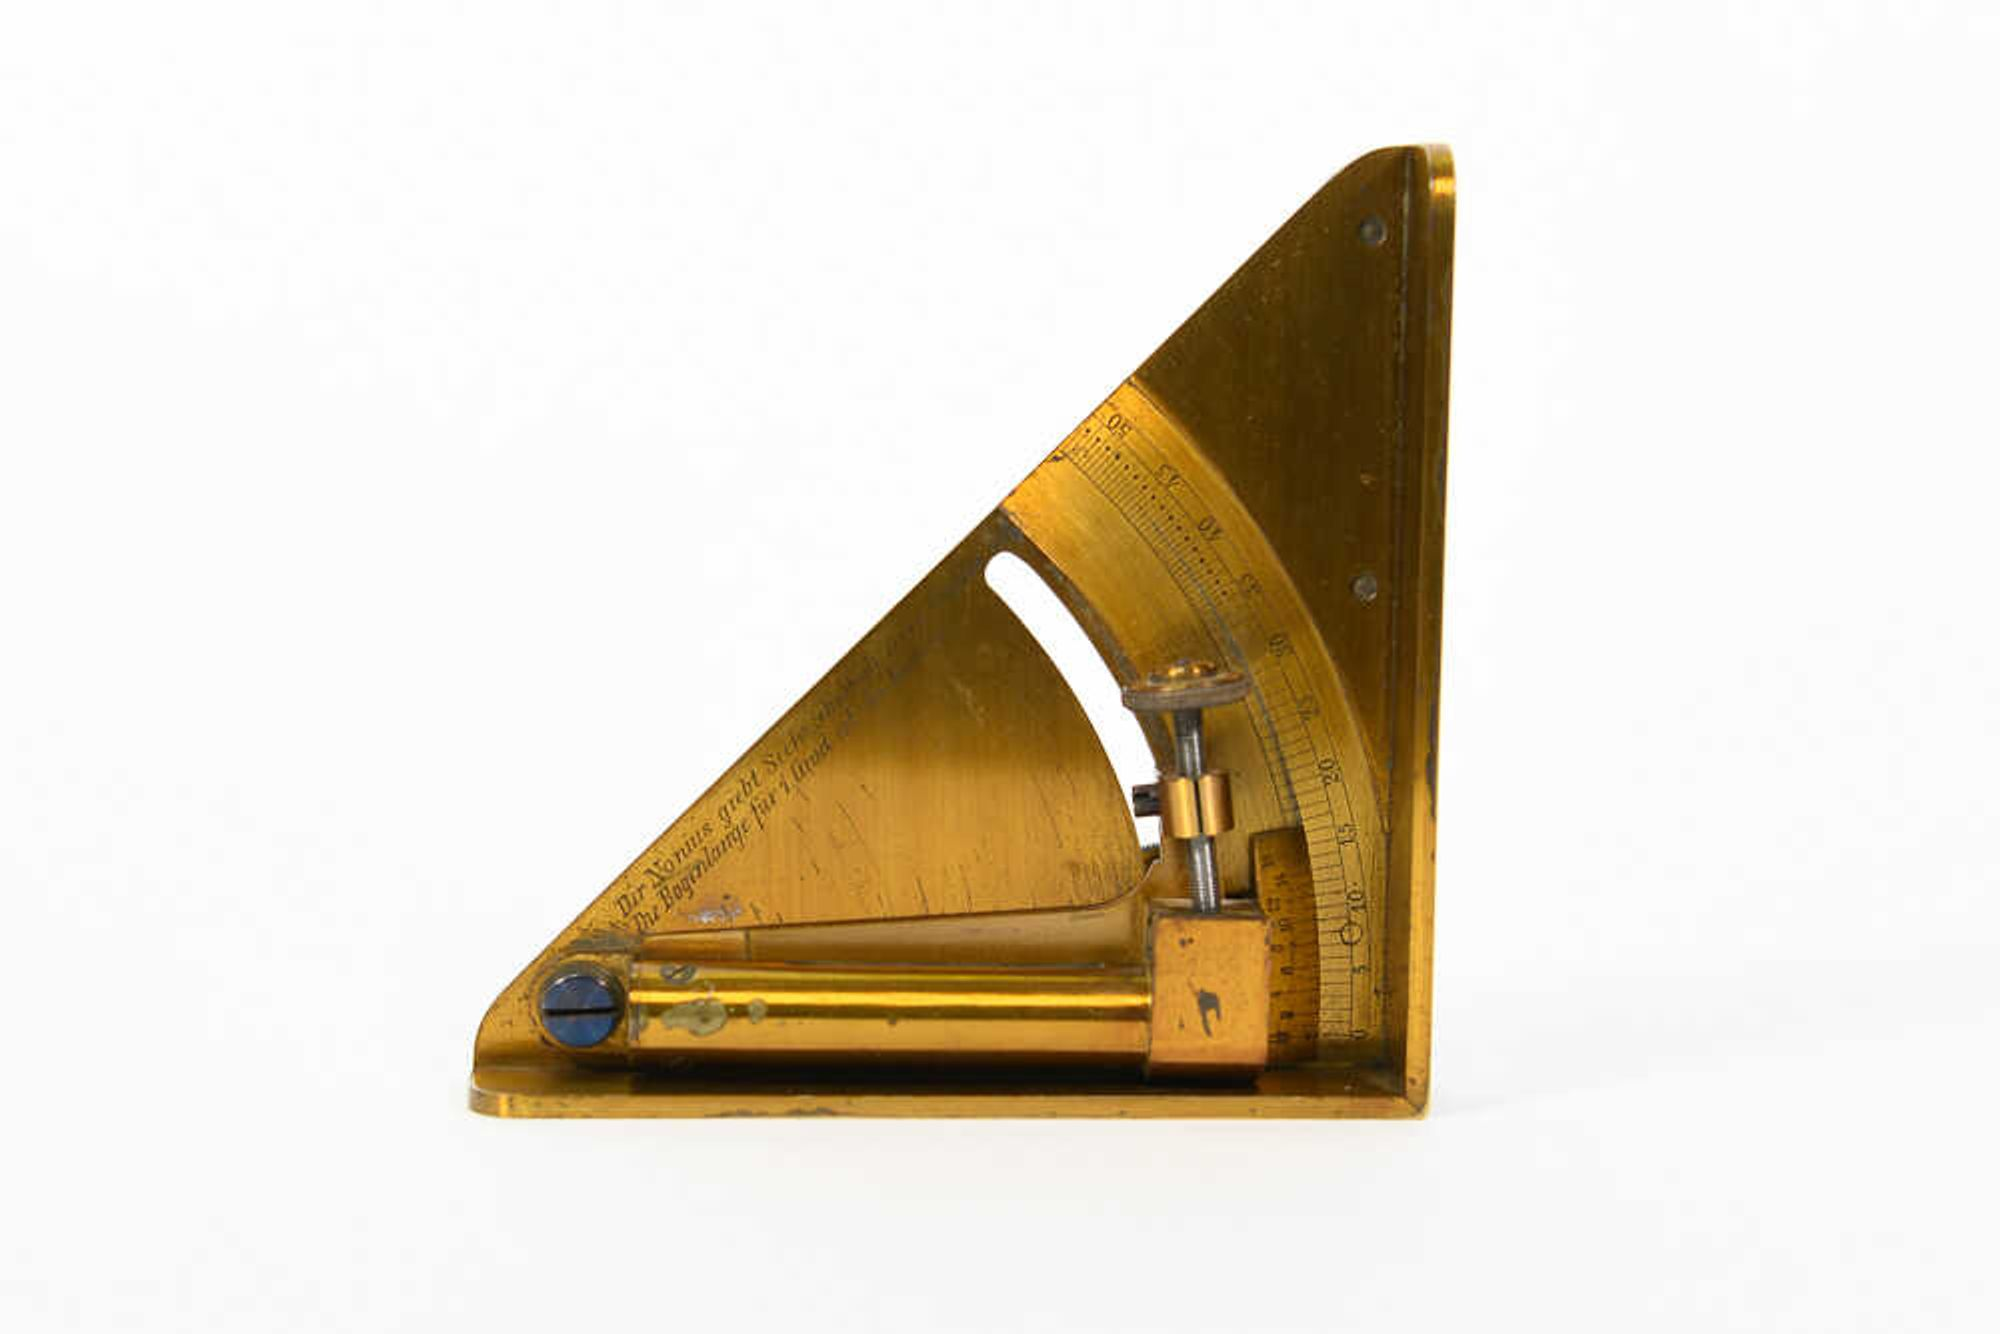
\includegraphics[width=0.8\textwidth]{img/21090101.jpg}
            \caption{藏品图片\cite{馆藏目录}}
            \label{fig:raw_pic}
        \end{figure}
\end{itemize}

\section{仪器描述}

\subsection{仪器外观}

\subsubsection{盒子}

此测斜仪由外部的盒子和内部的测量仪组成。盒子为皮质,内部的测量仪大部分为黄铜(铜、锌合金),少部分为钢。部分组件由玻璃制成,内含液体,可能为酒精。\cite{Clinometer}

如图\ref{fig:box_surface}所示,盒子为三角形的形状,旁边有两个铜制卡扣。通过旋转的方式解开卡扣后,可以沿着长边打开盒子。盒子外表面为黑色,边缘及角落磨损较严重,能看见内部的黄色填充物,如图\ref{fig:box_surface_outside}。盒子内表面为浅黄色毛毡,有一些污渍,如图\ref{fig:box_surface_inside}。盒子内部有一些放置测量仪并辅助固定其部件的凹槽。

\begin{figure}[h]
    \centering
    \begin{minipage}[t]{0.33\textwidth}
        \centering
        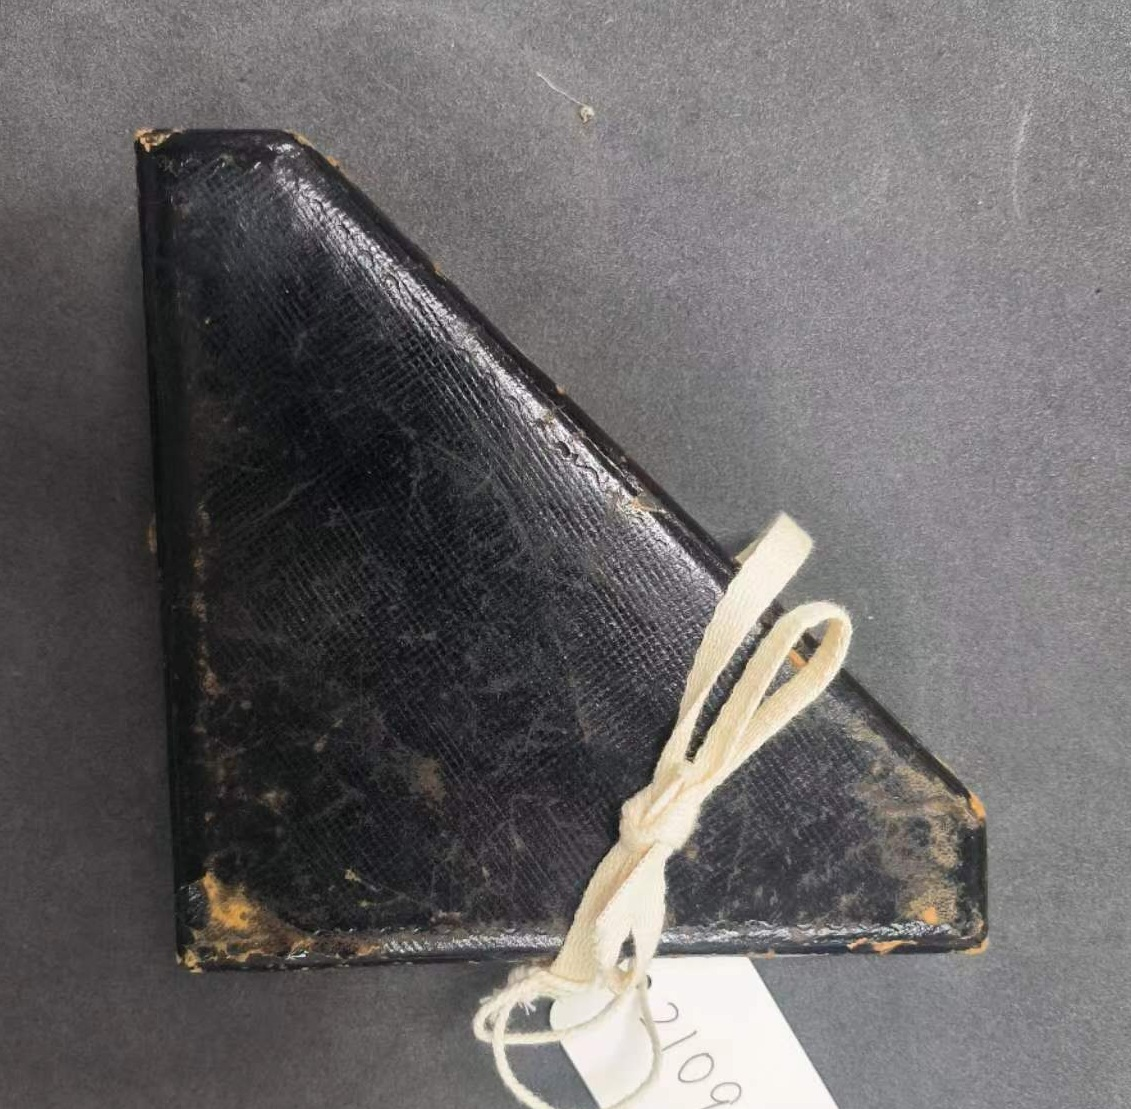
\includegraphics[width=0.8\textwidth]{img/box_surface.jpg}
        \caption{盒子外观}
    \label{fig:box_surface}
    \end{minipage}
    \begin{minipage}[t]{0.32\textwidth}
        \centering
        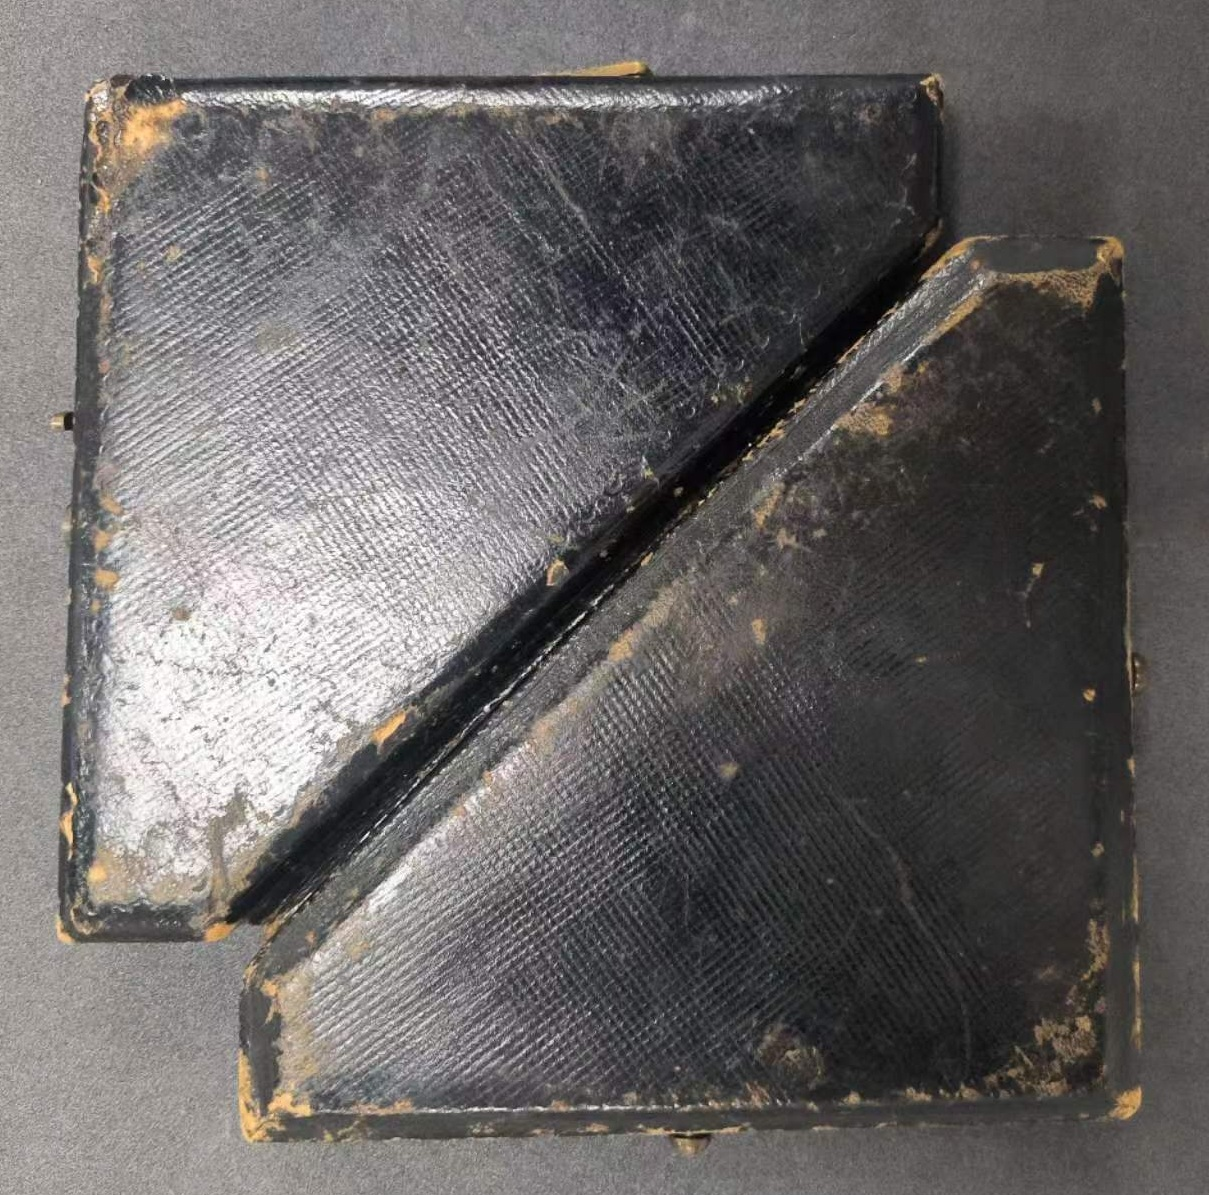
\includegraphics[width=0.8\textwidth]{img/box_surface_outside.jpg}
        \caption{盒子打开后的外部}
    \label{fig:box_surface_outside}
    \end{minipage}
    \begin{minipage}[t]{0.33\textwidth}
        \centering
        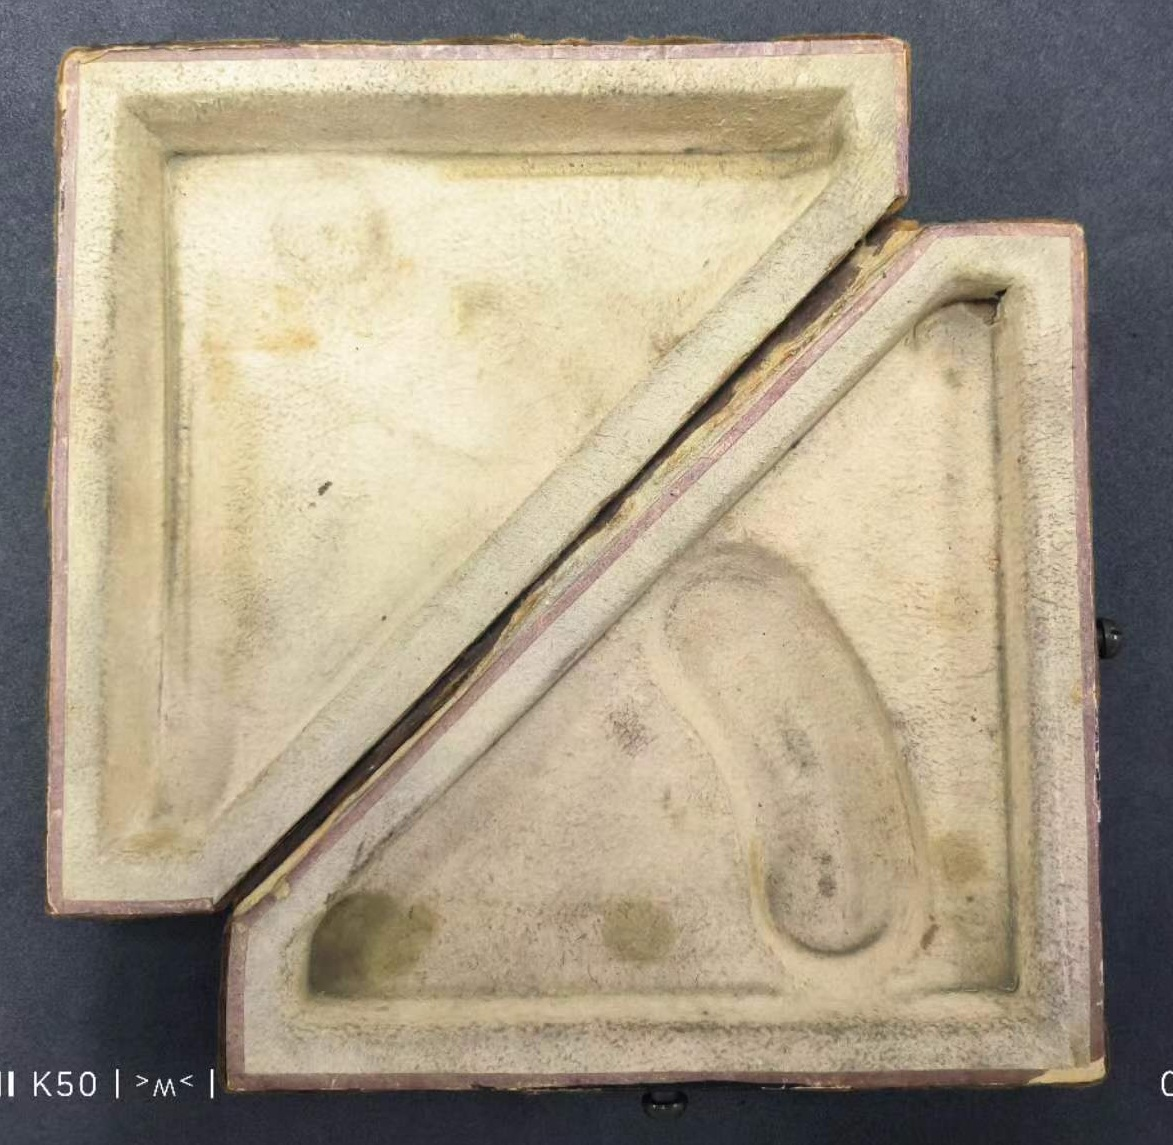
\includegraphics[width=0.8\textwidth]{img/box_surface_inside.jpg}
        \caption{盒子打开后的内部}
    \label{fig:box_surface_inside}
    \end{minipage}
\end{figure}

\subsubsection{测斜仪}

如图\ref{fig:clinometer_surface_face},测斜仪正面保存较为完好,表盘中有一定的空隙,长边可以看见一些刻字,内容为“Der Nonius giebt Sechszehntheile Theile eines Grades an. Die Bogenlänge für 1 Grad ist = 7/400 Radius.”,含义为:“游标表示十六分之一度。1 度的弧长 = 7/400 半径。”。表盘右侧可以看见测量所用的刻度。表盘正面能看见一些不可拆除的用于固定的螺丝。

如图\ref{fig:clinometer_surface_back},测量仪背面有明显使用与磨损痕迹,亦有刻字。顶部有花体的“F”与“L”:$\mathcal{F} \mathcal{L}$。“F”与“L”下方有小字,用花体刻着“1113”。左边也刻着“1113”,右侧尖角处刻着制作者的名字“W. Bandermann Berlin”。在这段话的左侧刻着“3679”,推测为代表第3679号产品\cite{laoxiangji}。背面亦可以看见多个不可拆除的用于固定的螺丝。

如图\ref{fig:clinometer_surface_left},测量仪侧面能看出少量使用痕迹,底部用于转轴的螺丝贴片稍有变形。在此处可观察用于测量的游标:游标内嵌一个玻璃管,内含液体和气泡。游标上有一些刻度,用于测量角度。

\begin{figure}[h]
    \centering
    \begin{minipage}[t]{0.38\textwidth}
        \centering
        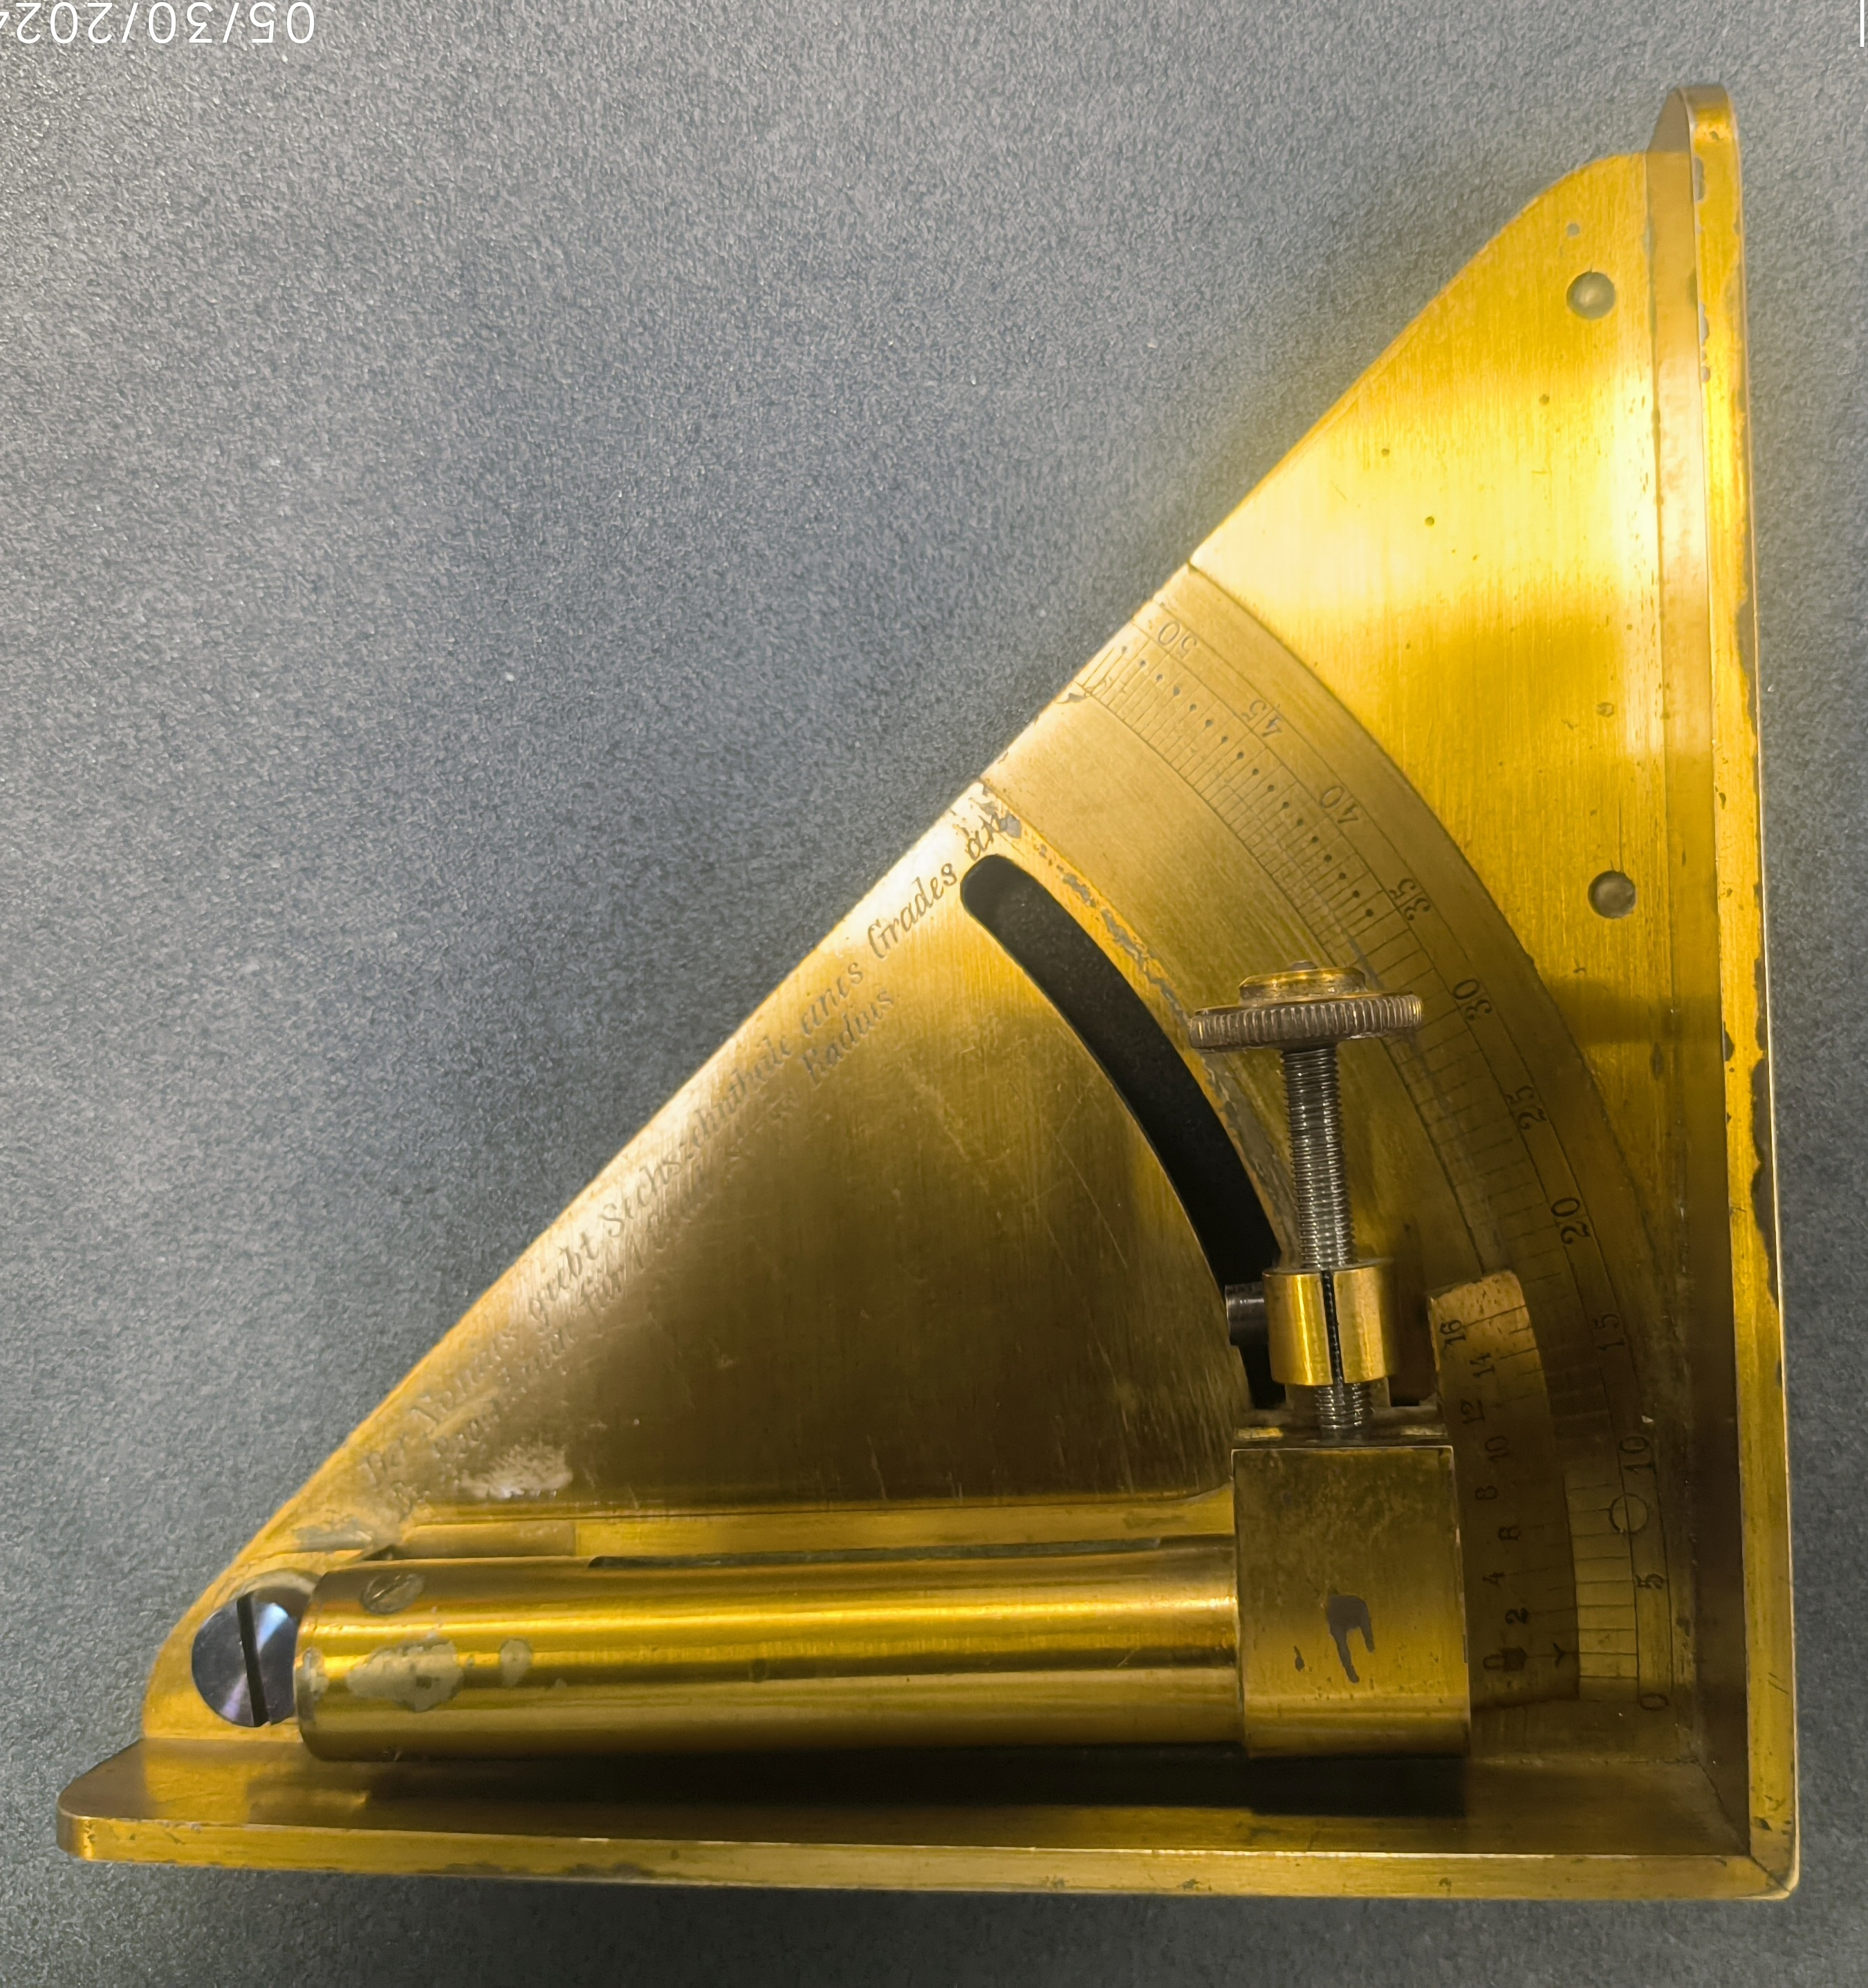
\includegraphics[width=0.75\textwidth]{img/clinometer_surface_face.jpg}
        \caption{测斜仪正面}
    \label{fig:clinometer_surface_face}
    \end{minipage}
    \begin{minipage}[t]{0.38\textwidth}
        \centering
        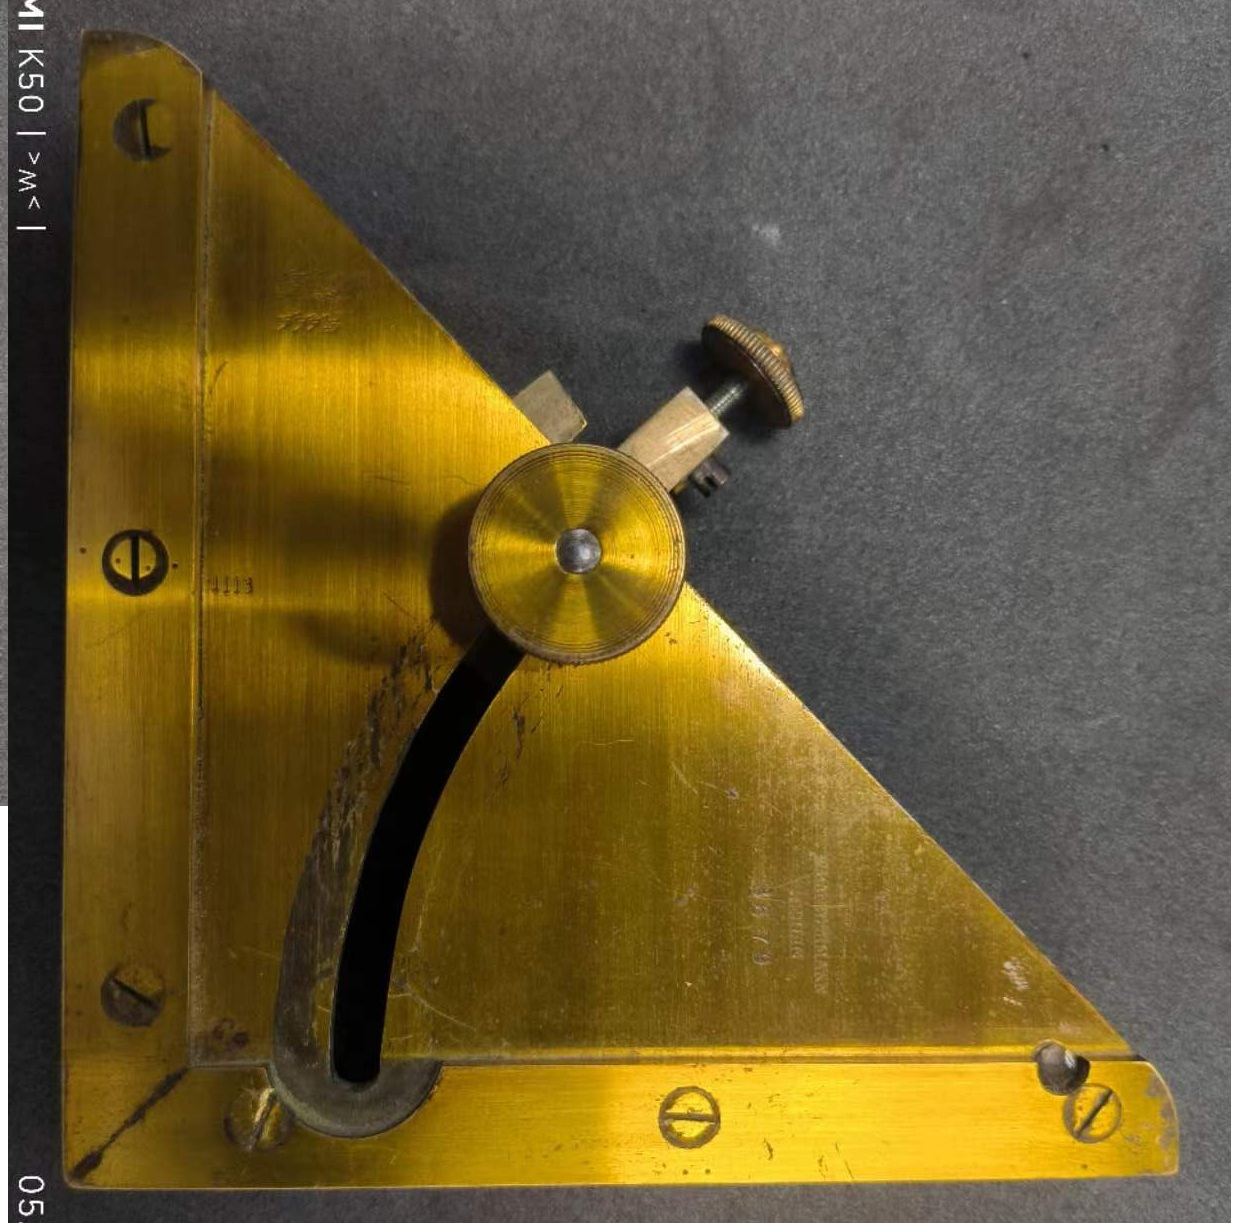
\includegraphics[width=0.8\textwidth]{img/clinometer_surface_back.jpg}
        \caption{测斜仪背面}
    \label{fig:clinometer_surface_back}
    \end{minipage}
    \begin{minipage}[t]{0.2\textwidth}
        \centering
        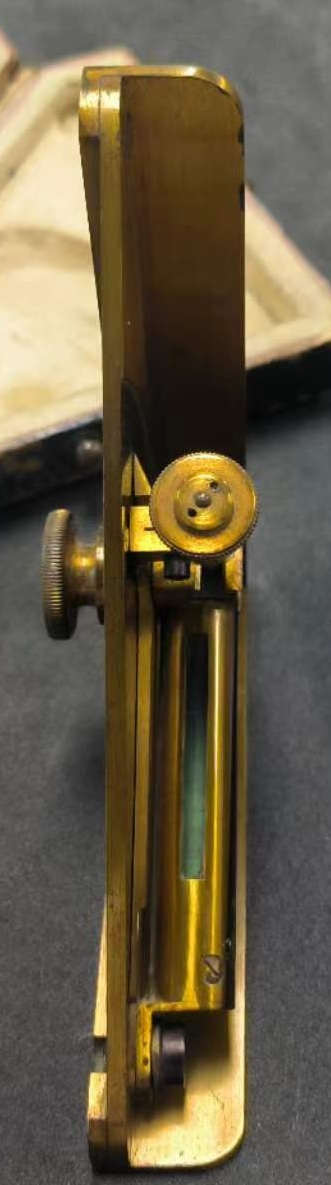
\includegraphics[width=0.42\textwidth]{img/clinometer_surface_left.jpg}
        \caption{测斜仪左侧}
    \label{fig:clinometer_surface_left}
    \end{minipage}
\end{figure}

\subsection{仪器结构与参数}

\subsubsection{盒子}

用于放置仪器的皮革盒子呈正方形剪去等腰直角三角形的五边形形状(如图\ref{fig:box_surface_measure}),边长 136.0 mm,凸出部分长 26.0 mm,厚41.0 mm。重150 g。盒子的两面直接由皮革连接,无铰链等连接件。

\begin{figure}[h]
    \centering
    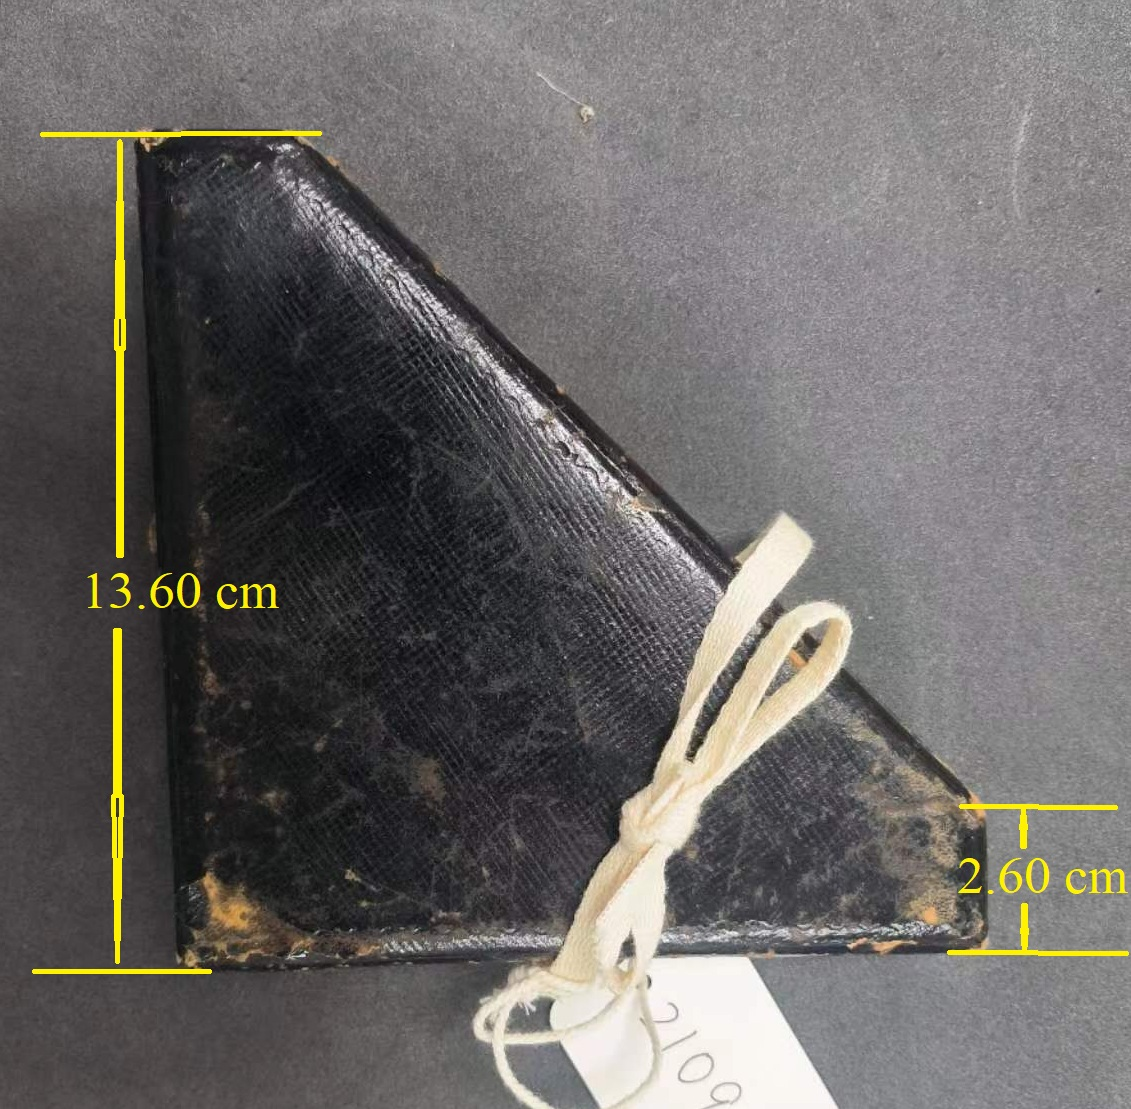
\includegraphics[width=0.4\textwidth]{img/box_surface_measure.jpg}
    \caption{盒子尺寸测量}
    \label{fig:box_surface_measure}
\end{figure}

\subsubsection{测斜仪}

测量仪整体长 112.6 mm, 宽 112.6 mm,厚 23.0 mm,重量为 420 g。测量仪主要由底座(用于保护测量的盘)、量盘、游标组成。底座为一个支架与量盘由 6 个螺钉或榫卯固定(每条直角边均匀分布 3 个螺钉或铆钉),不可拆卸。

如图\ref{fig:clinometer_structure_face_undisassembled},游标和量盘通过两个螺丝连接,位于根部(绿色圈内)的小螺丝作为支点,小螺丝与游标之间有一个变形的金属片,用于提供阻尼。位于尾部(蓝色圈内)的大螺丝用于调整游标的角度,以及用于调整游标的角度的时候提供阻尼。

\begin{figure}[h]
    \centering
    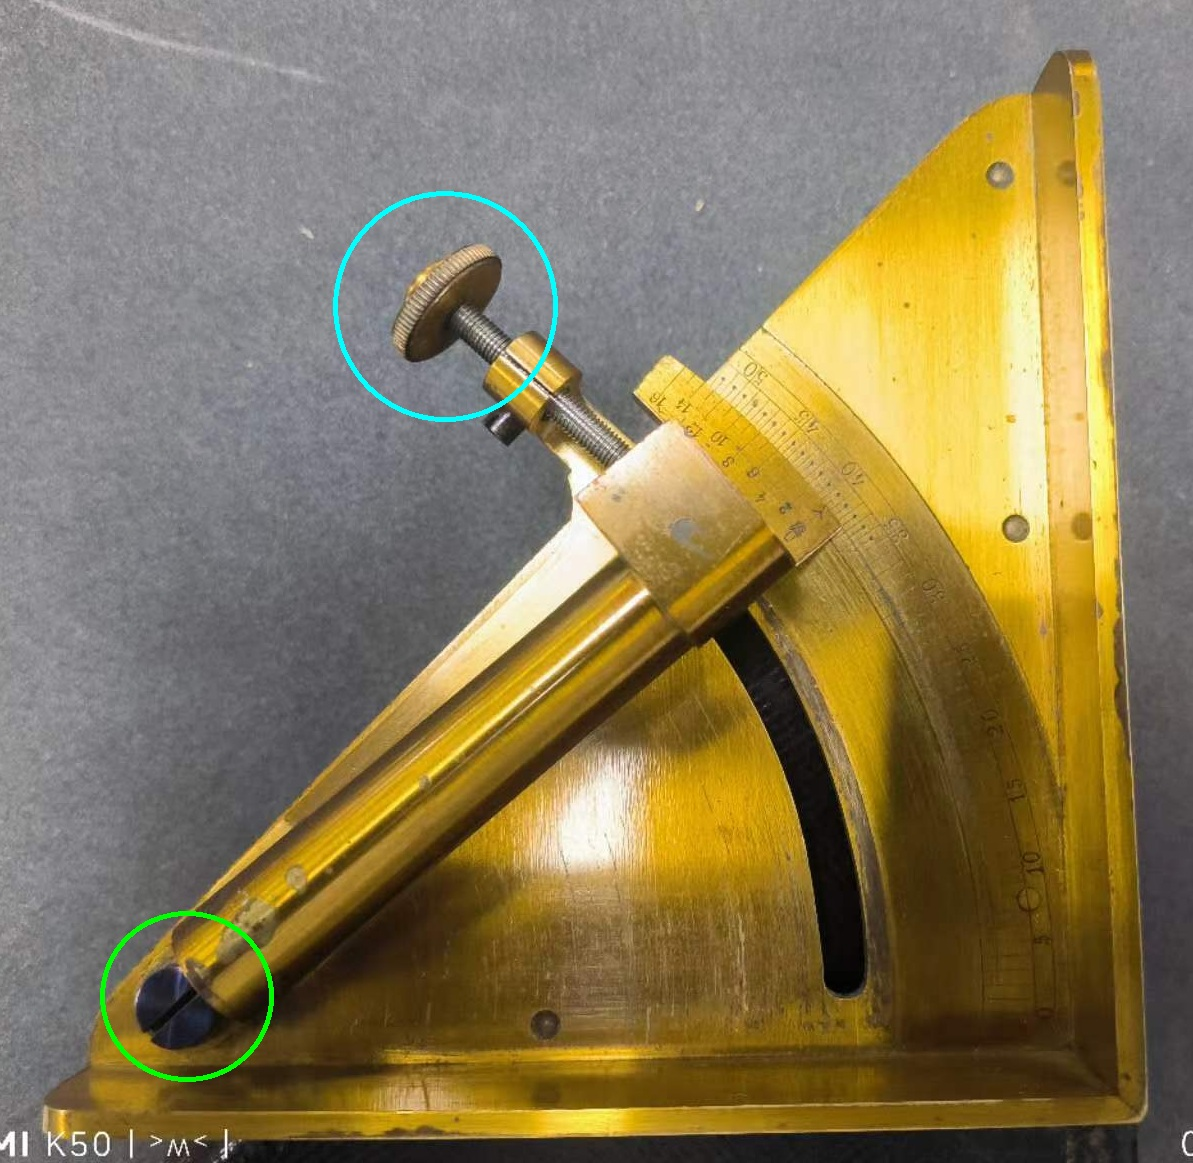
\includegraphics[width=0.4\textwidth]{img/clinometer_structure_face_undisassembled}
    \caption{测斜仪结构}
    \label{fig:clinometer_structure_face_undisassembled}
\end{figure}

\subsubsection{量盘}

拆掉游标后,可以看见完整的量盘。如图\ref{fig:clinometer_structure_face_disassembled},量盘正面有刻度,用于读取角度。量盘的量程为0°-52°。在0°-30°之间,每两个大刻度间为1°,没有小刻度。在30°-52°之间,每两个大刻度中间有一个小刻度,刻度之间间隔为0.5°。游标上有16个小刻度,和量盘一起使用,可以测量1°的十六分之一(在大于30°的时候,由于游标超出量盘,可以取半个游标使用,测量0.5°的八分之一)。量盘背面有由于游标的摩擦的明显痕迹。

\begin{figure}[h]
    \centering
    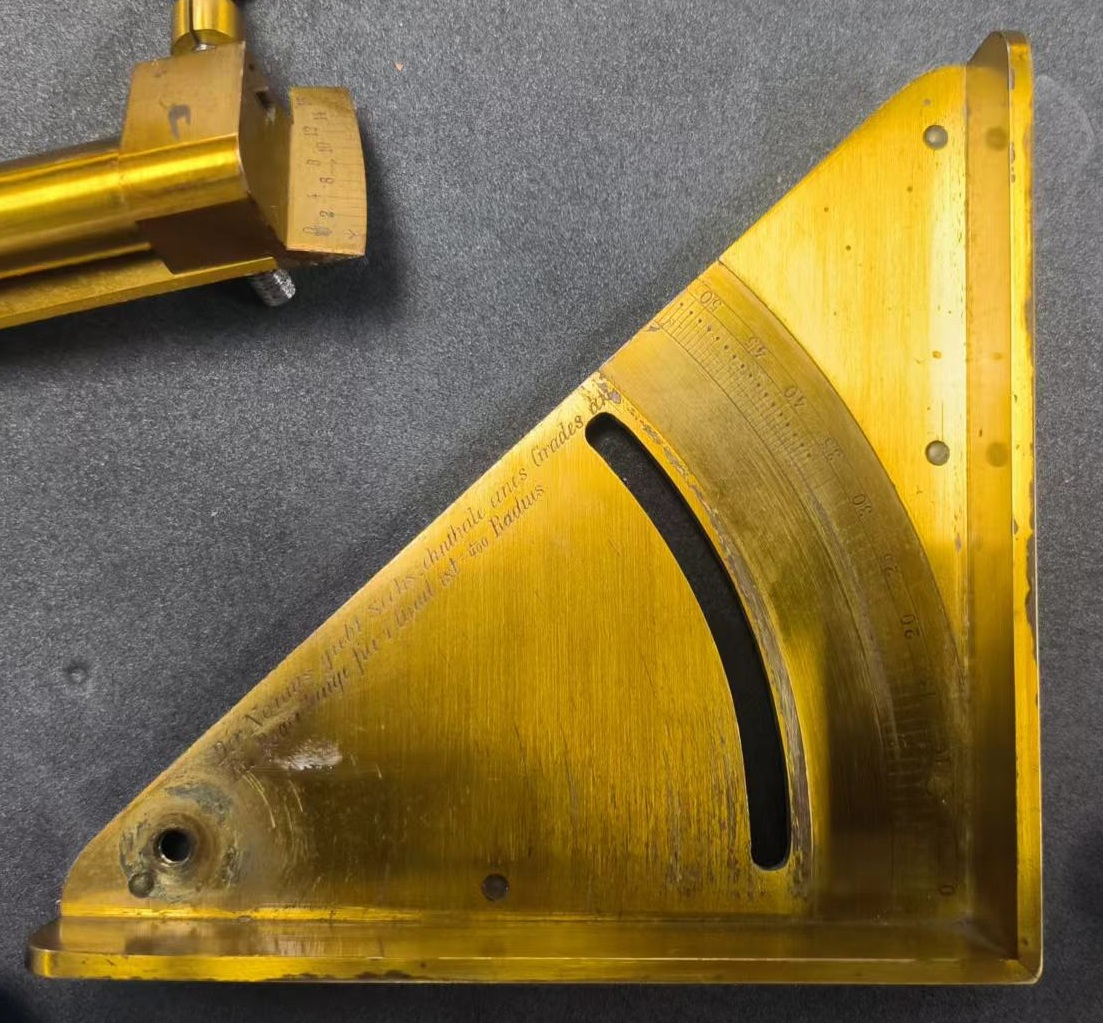
\includegraphics[width=0.4\textwidth]{img/clinometer_structure_face_disassembled}
    \caption{拆除游标后的量盘}
    \label{fig:clinometer_structure_face_disassembled}
\end{figure}

根据实际使用与测量,测斜仪能测量的最大角度为47°15',最小角度为-15'。由于游标最小值超出量盘量程,因此最小角度因为0°。即测斜仪的量程为0°-47°15'。

\subsubsection{游标}

游标可以拆卸为三部分,分别为游标底座、游标本体和螺帽。螺帽位于量盘背,与游标底座通过游标底部固定的螺丝连接。如图\ref{fig:vernier_structure_front}与图\ref{fig:vernier_structure_back},红色圈内的即为螺帽。游标背面的螺帽可以扭动,以调整游标的阻尼,以及拆卸游标。

\begin{figure}[h]
    \centering
    \begin{minipage}[t]{0.3\textwidth}
        \centering
        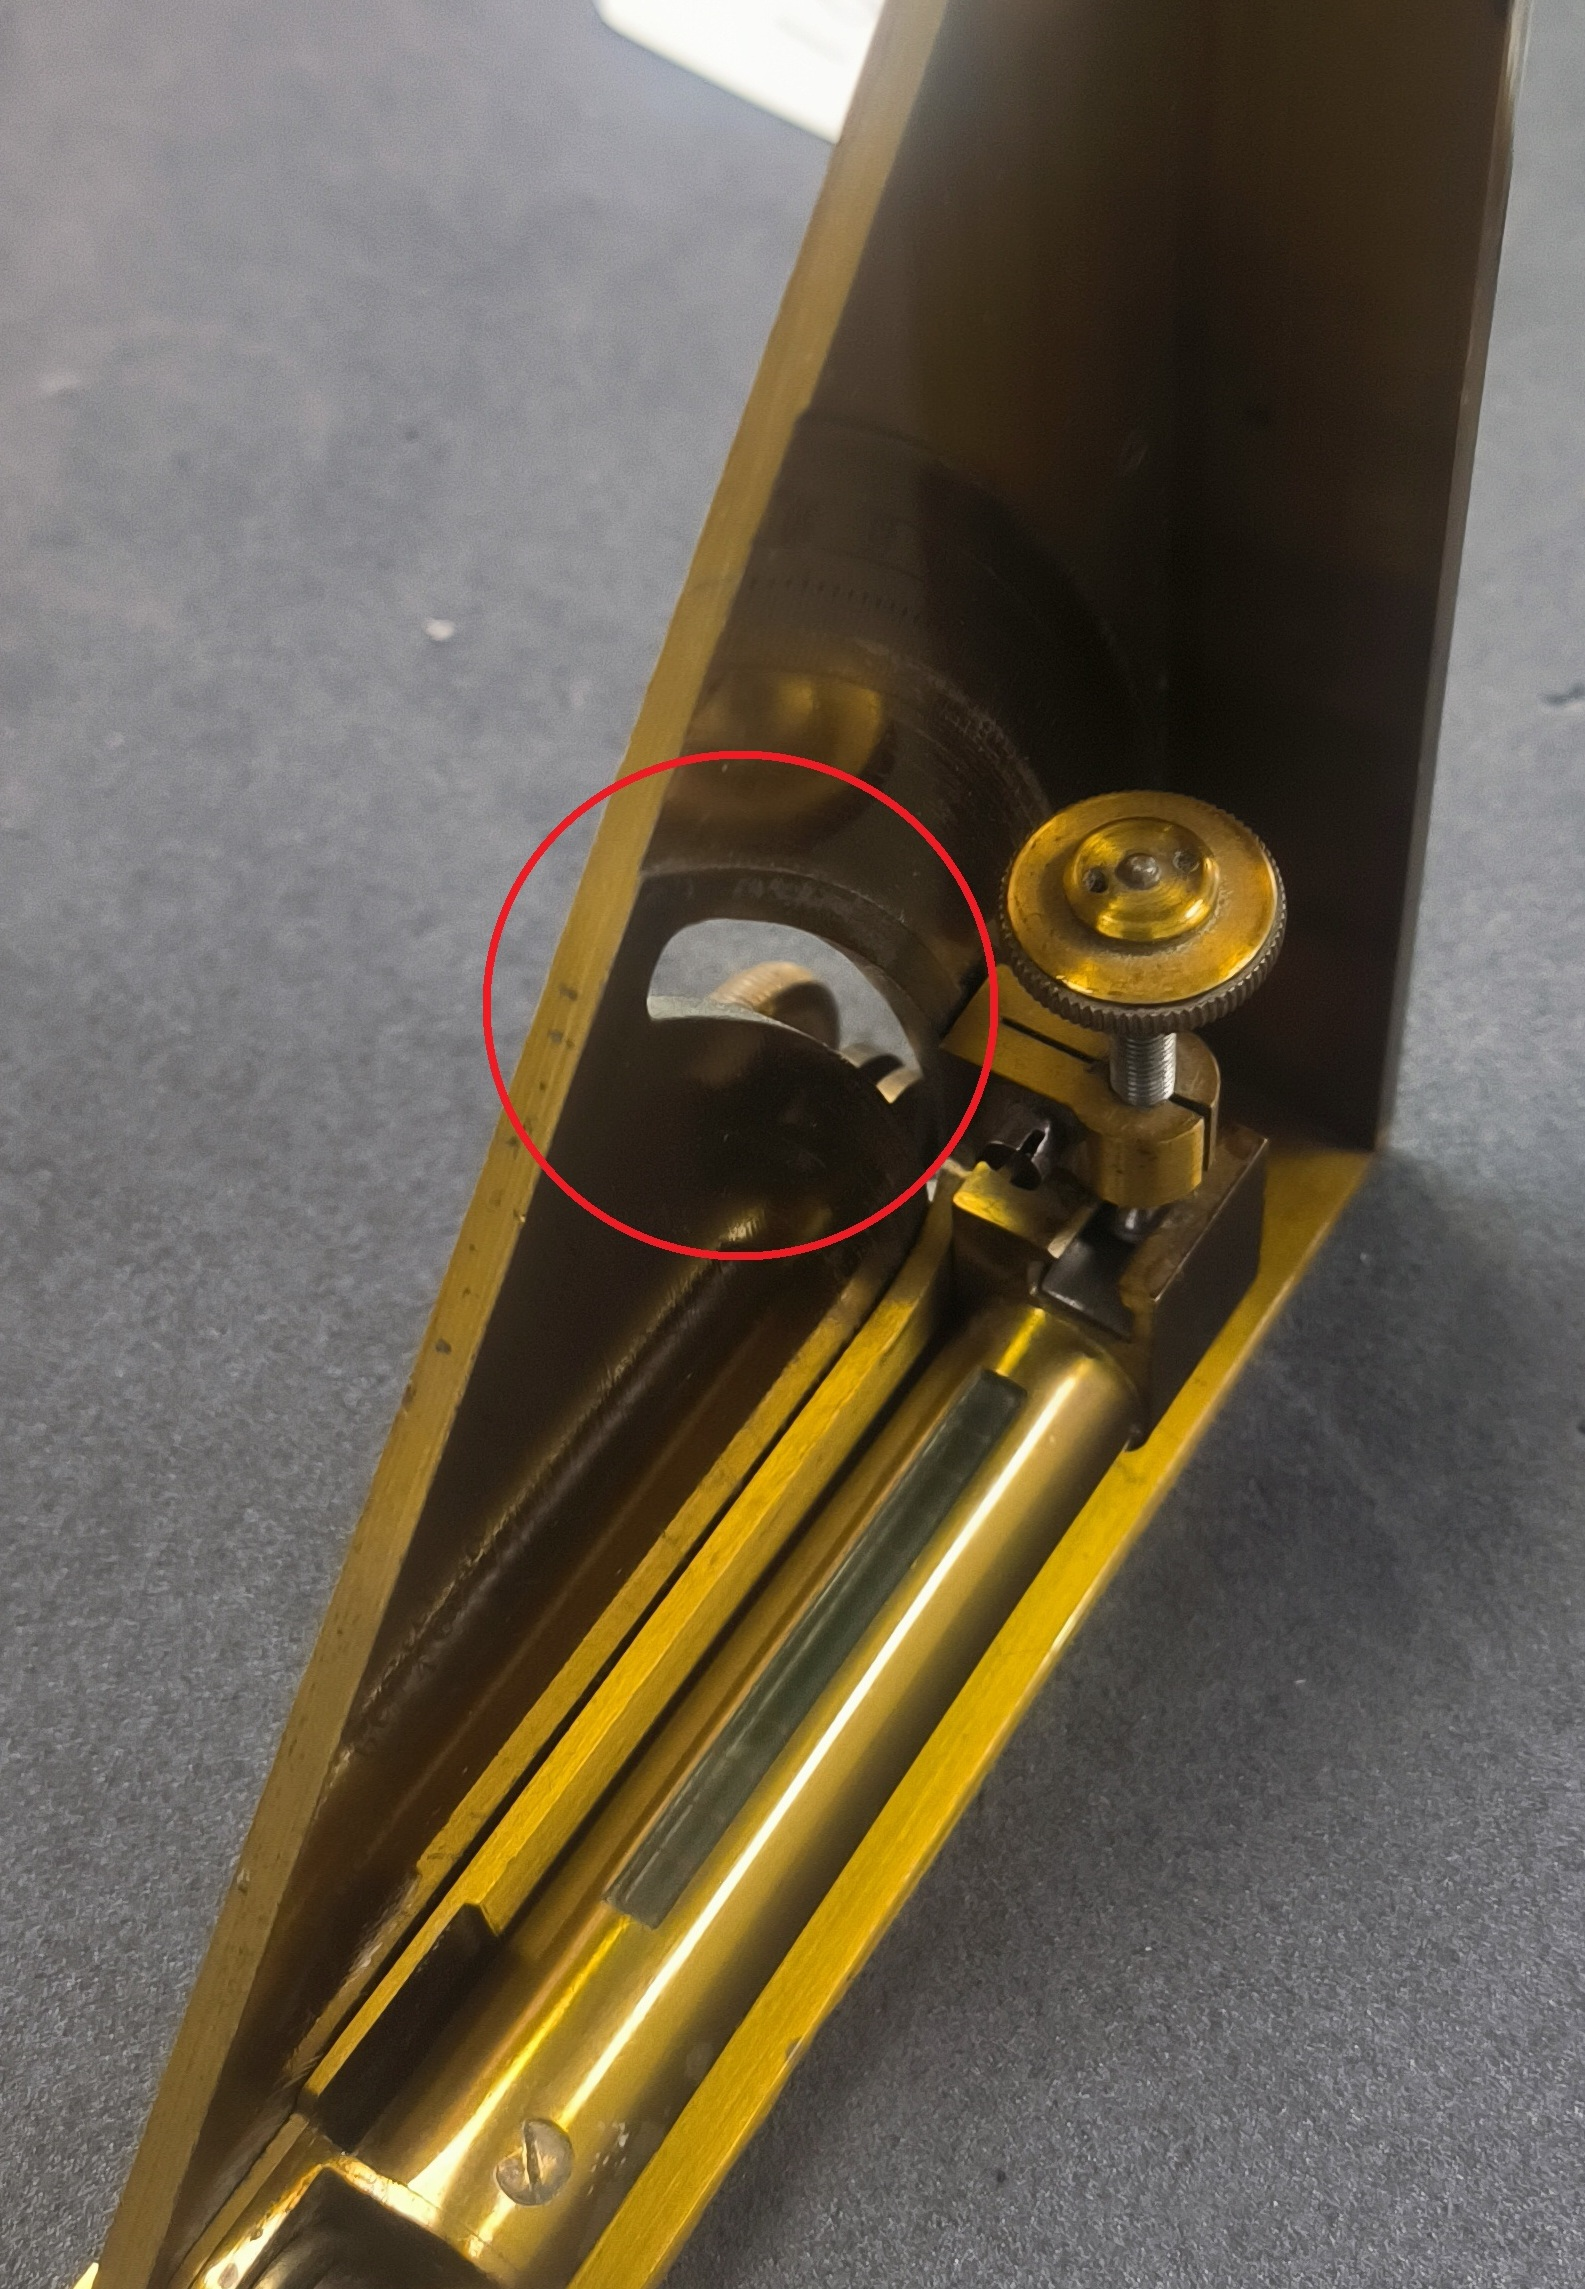
\includegraphics[width=0.8\textwidth]{img/vernier_structure_front.jpg}
        \caption{游标正面}
        \label{fig:vernier_structure_front}
    \end{minipage}
    \begin{minipage}[t]{0.3\textwidth}
        \centering
        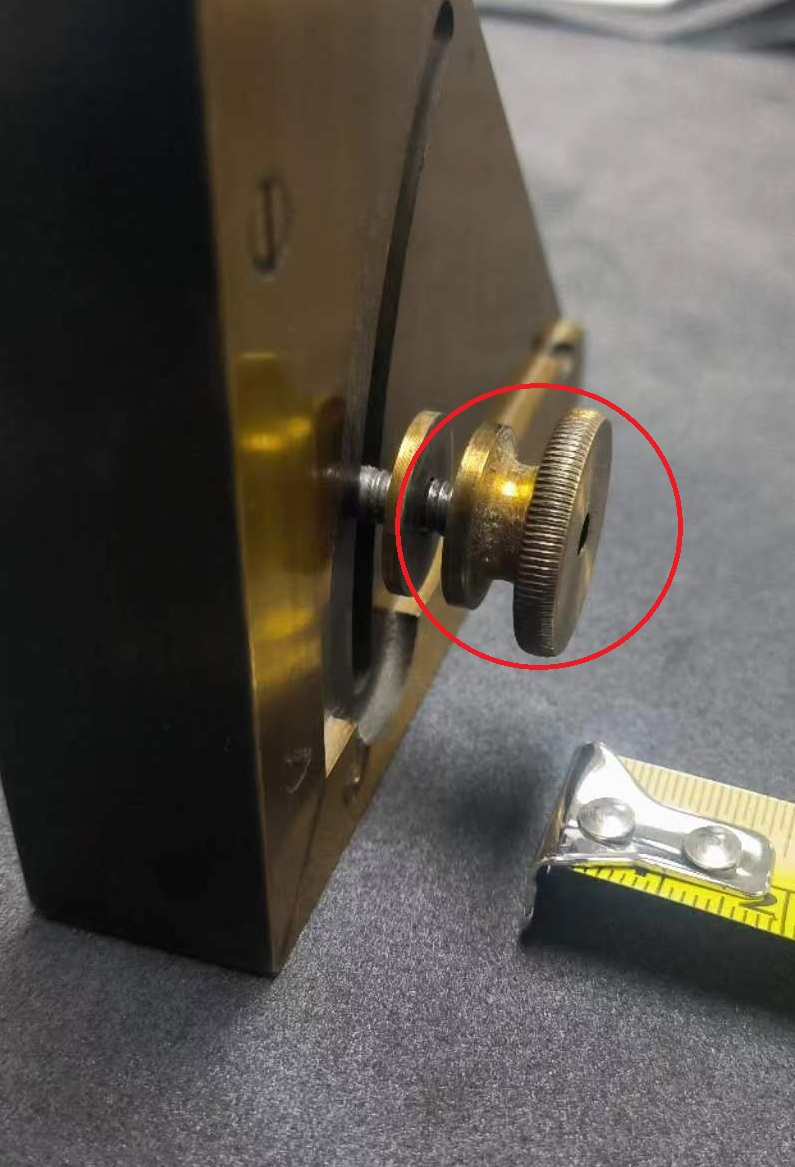
\includegraphics[width=0.78\textwidth]{img/vernier_structure_back.jpg}
        \caption{游标背面}
        \label{fig:vernier_structure_back}
    \end{minipage}
\end{figure}

如图\ref{fig:vernier_structure_disassembled},游标底座与游标本体通过机械结构拼接。如图图\ref{fig:vernier_structure_toassembled},可以将游标本体向左方插入,对齐两孔并锁住,即可组合成图\ref{fig:vernier_structure_assembled}的形状。此时套入量盘,旋紧游标根部的螺丝,并旋紧游标背面的螺帽,调整到合适的阻尼,即可使用。

\begin{figure}[h]
    \centering
    \begin{minipage}[t]{0.3\textwidth}
        \centering
        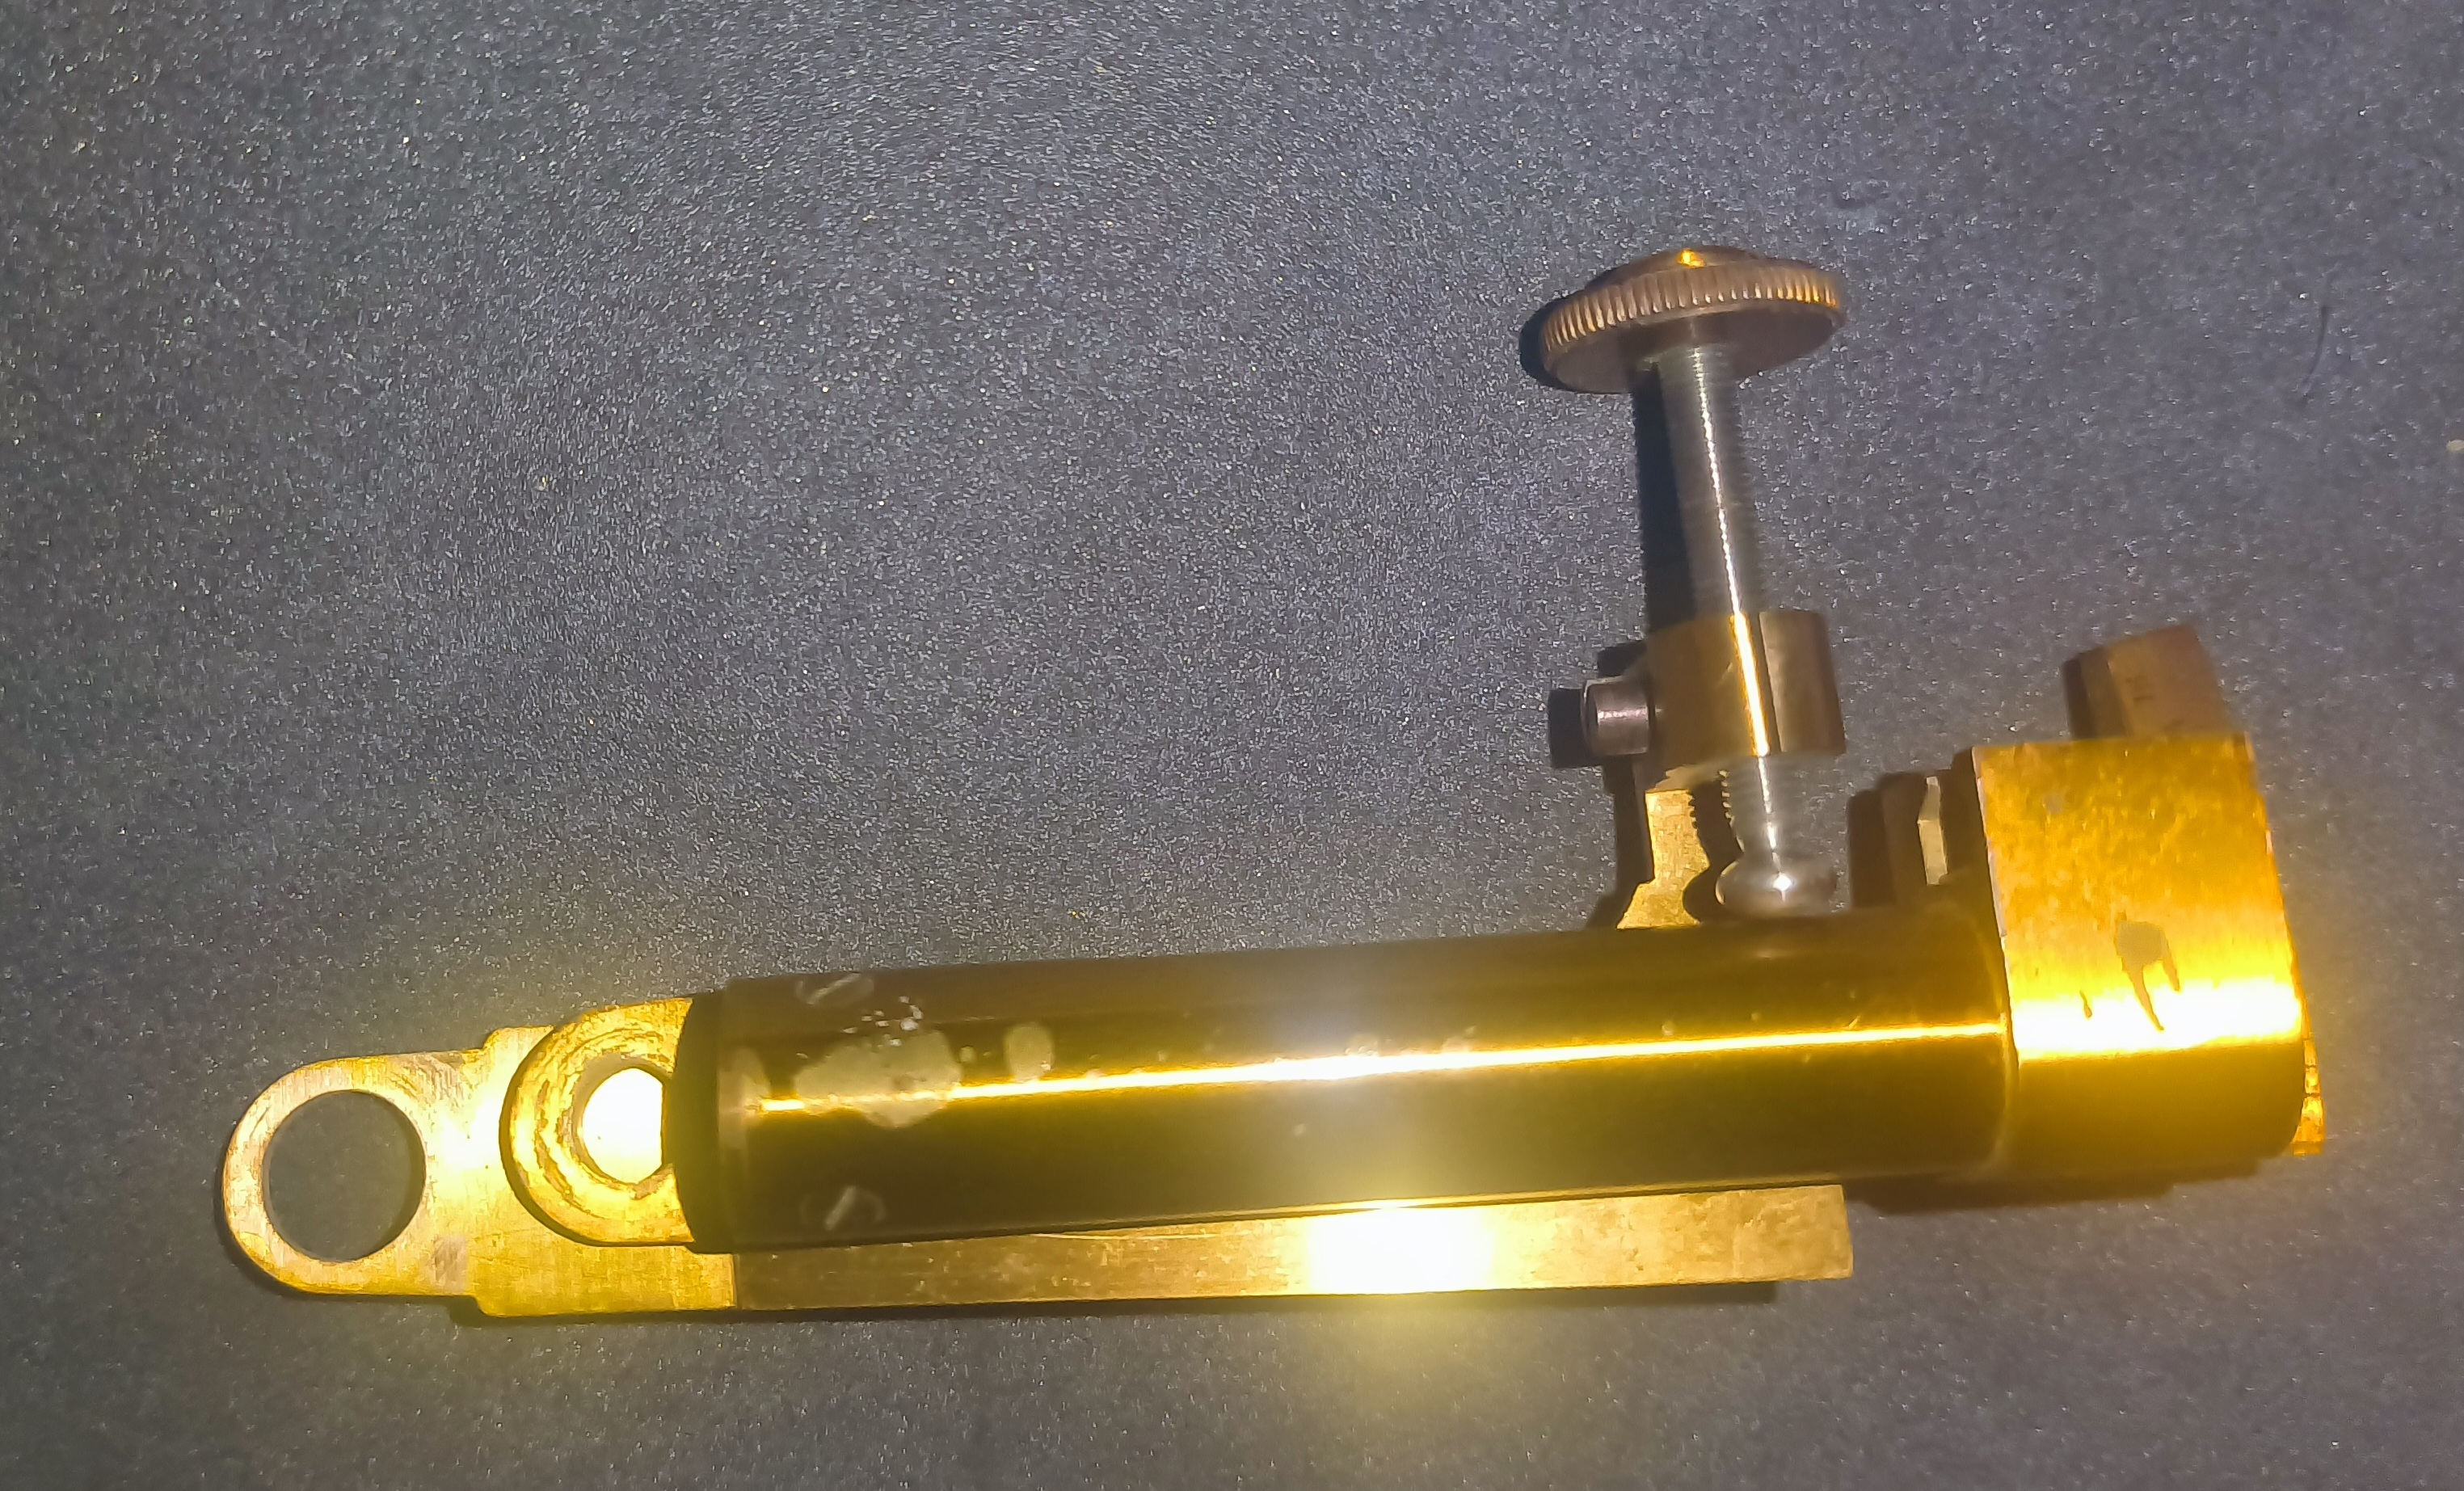
\includegraphics[width=0.9\textwidth]{img/vernier_structure_disassembled.jpg}
        \caption{拼接前}
        \label{fig:vernier_structure_disassembled}
    \end{minipage}
    \begin{minipage}[t]{0.3\textwidth}
        \centering
        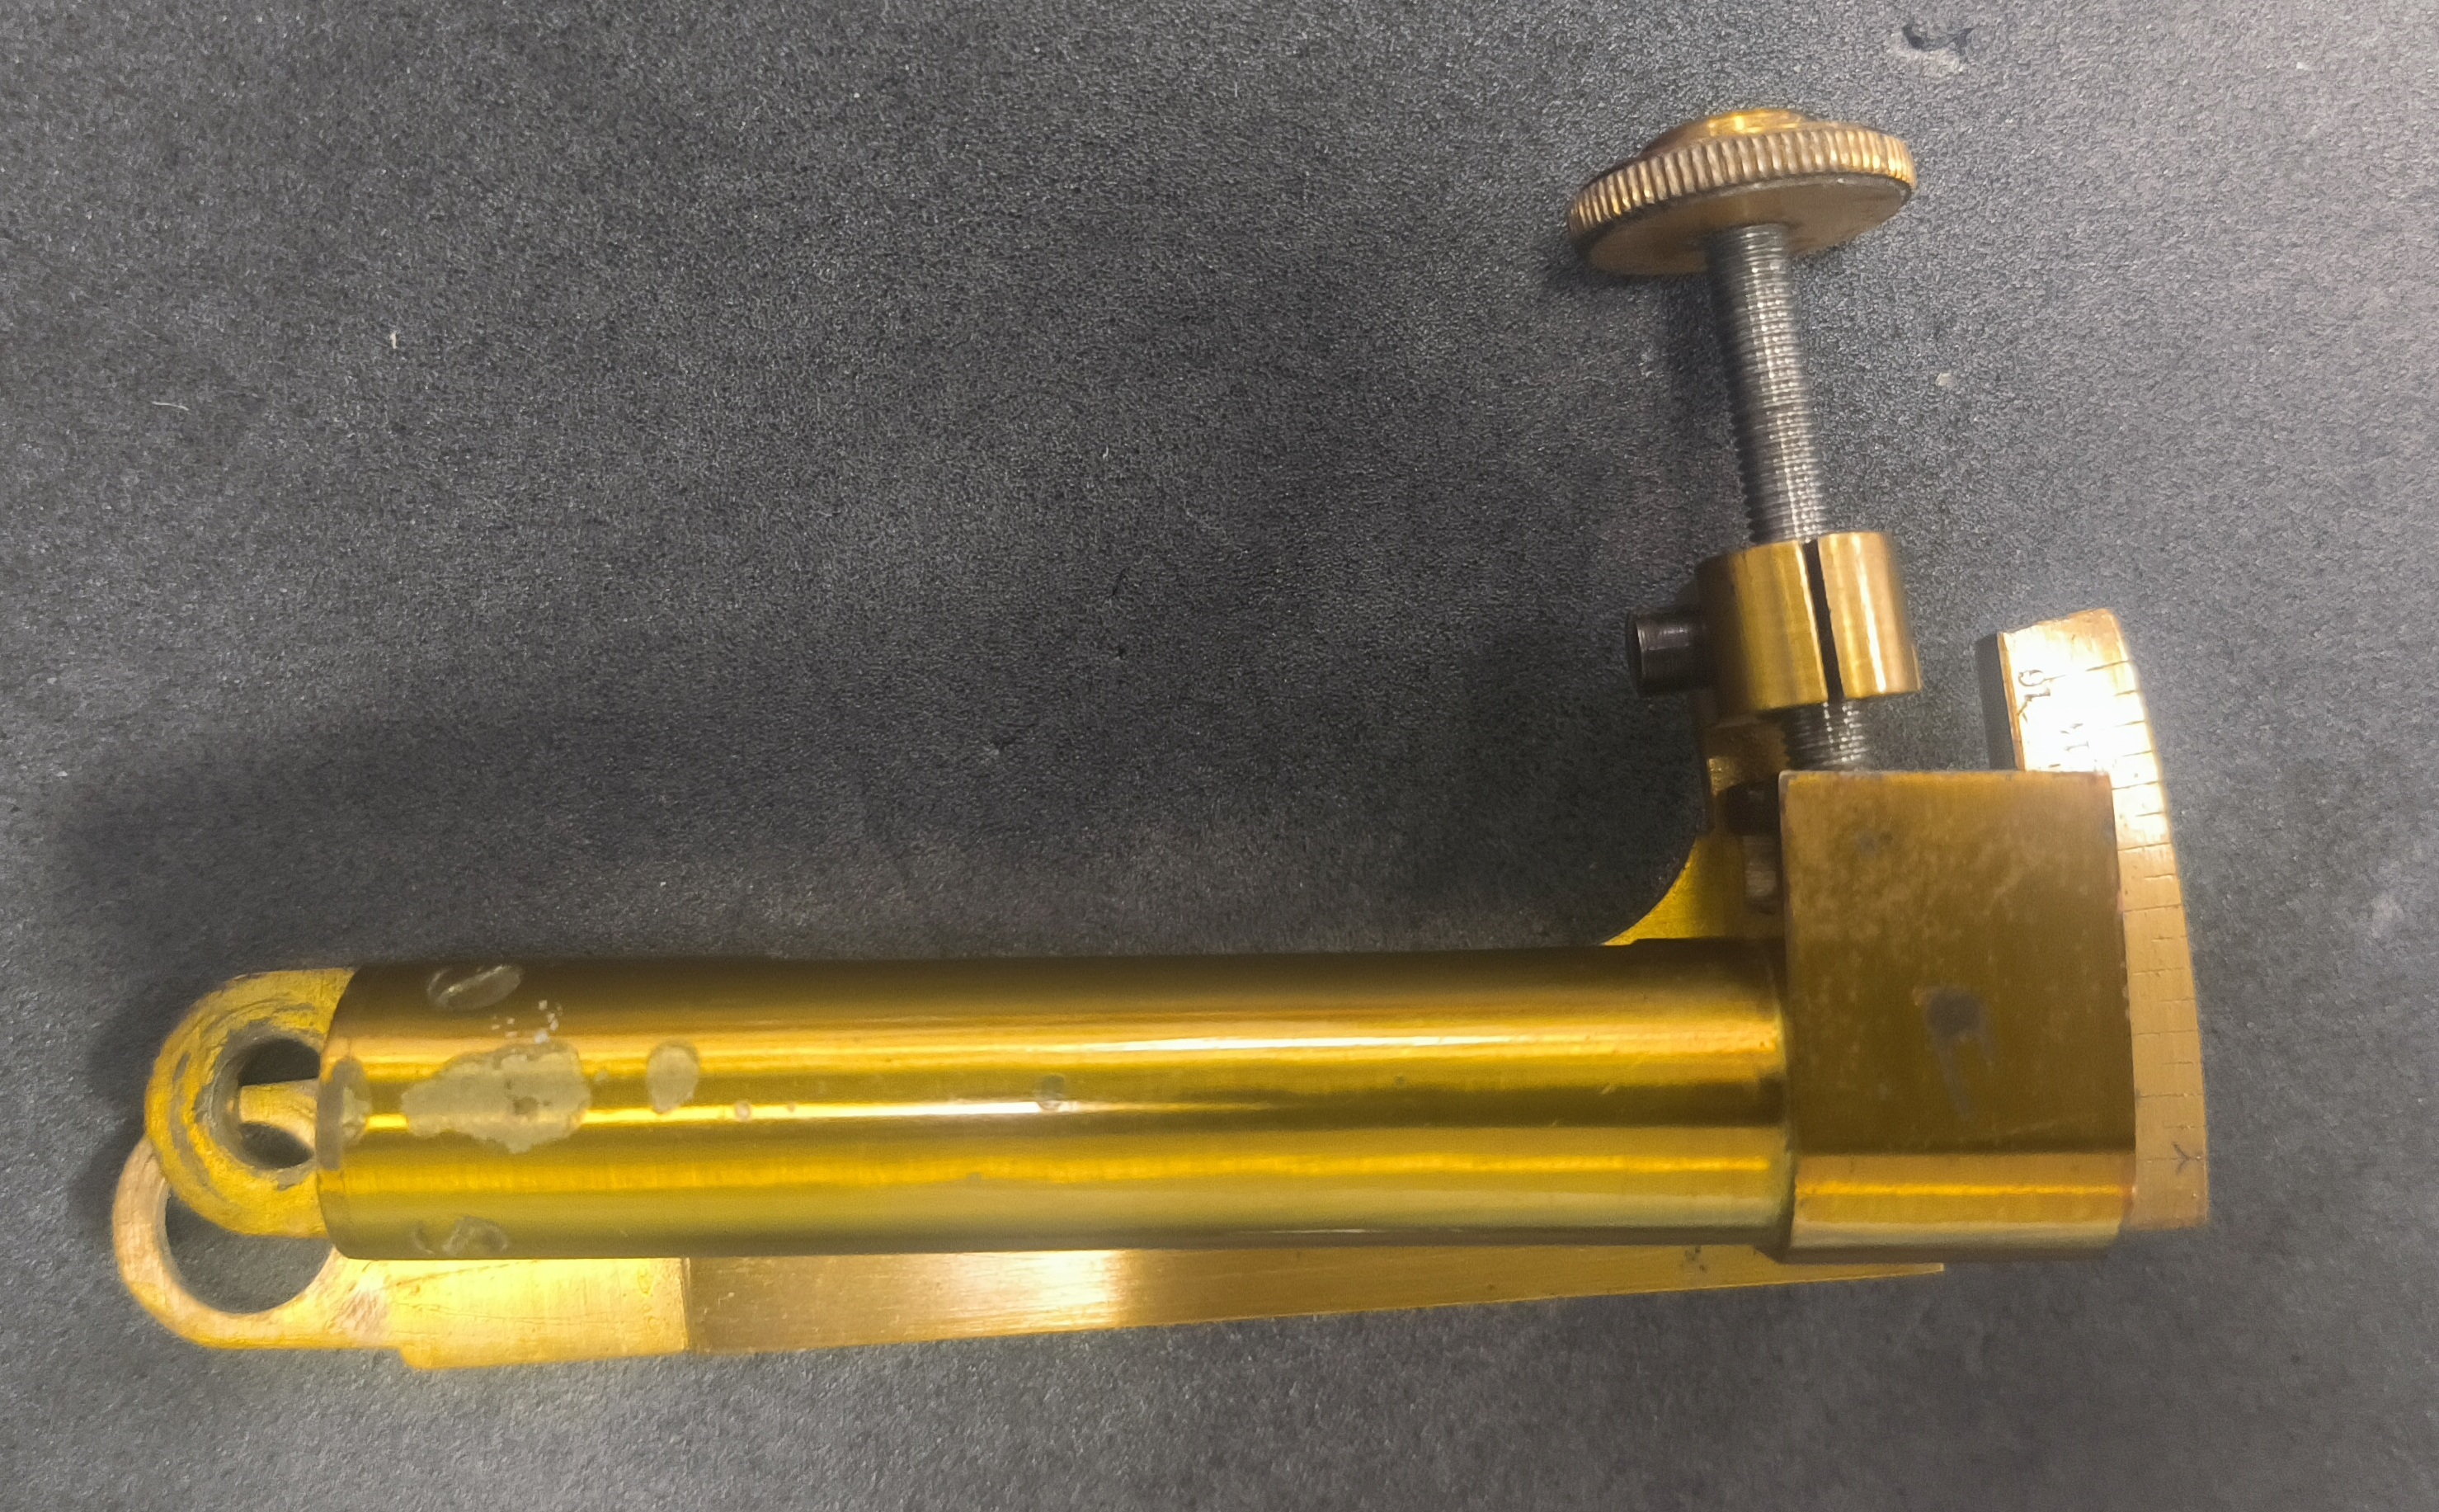
\includegraphics[width=0.87\textwidth]{img/vernier_structure_toassembled.jpg}
        \caption{拼接时}
        \label{fig:vernier_structure_toassembled}
    \end{minipage}
    \begin{minipage}[t]{0.3\textwidth}
        \centering
        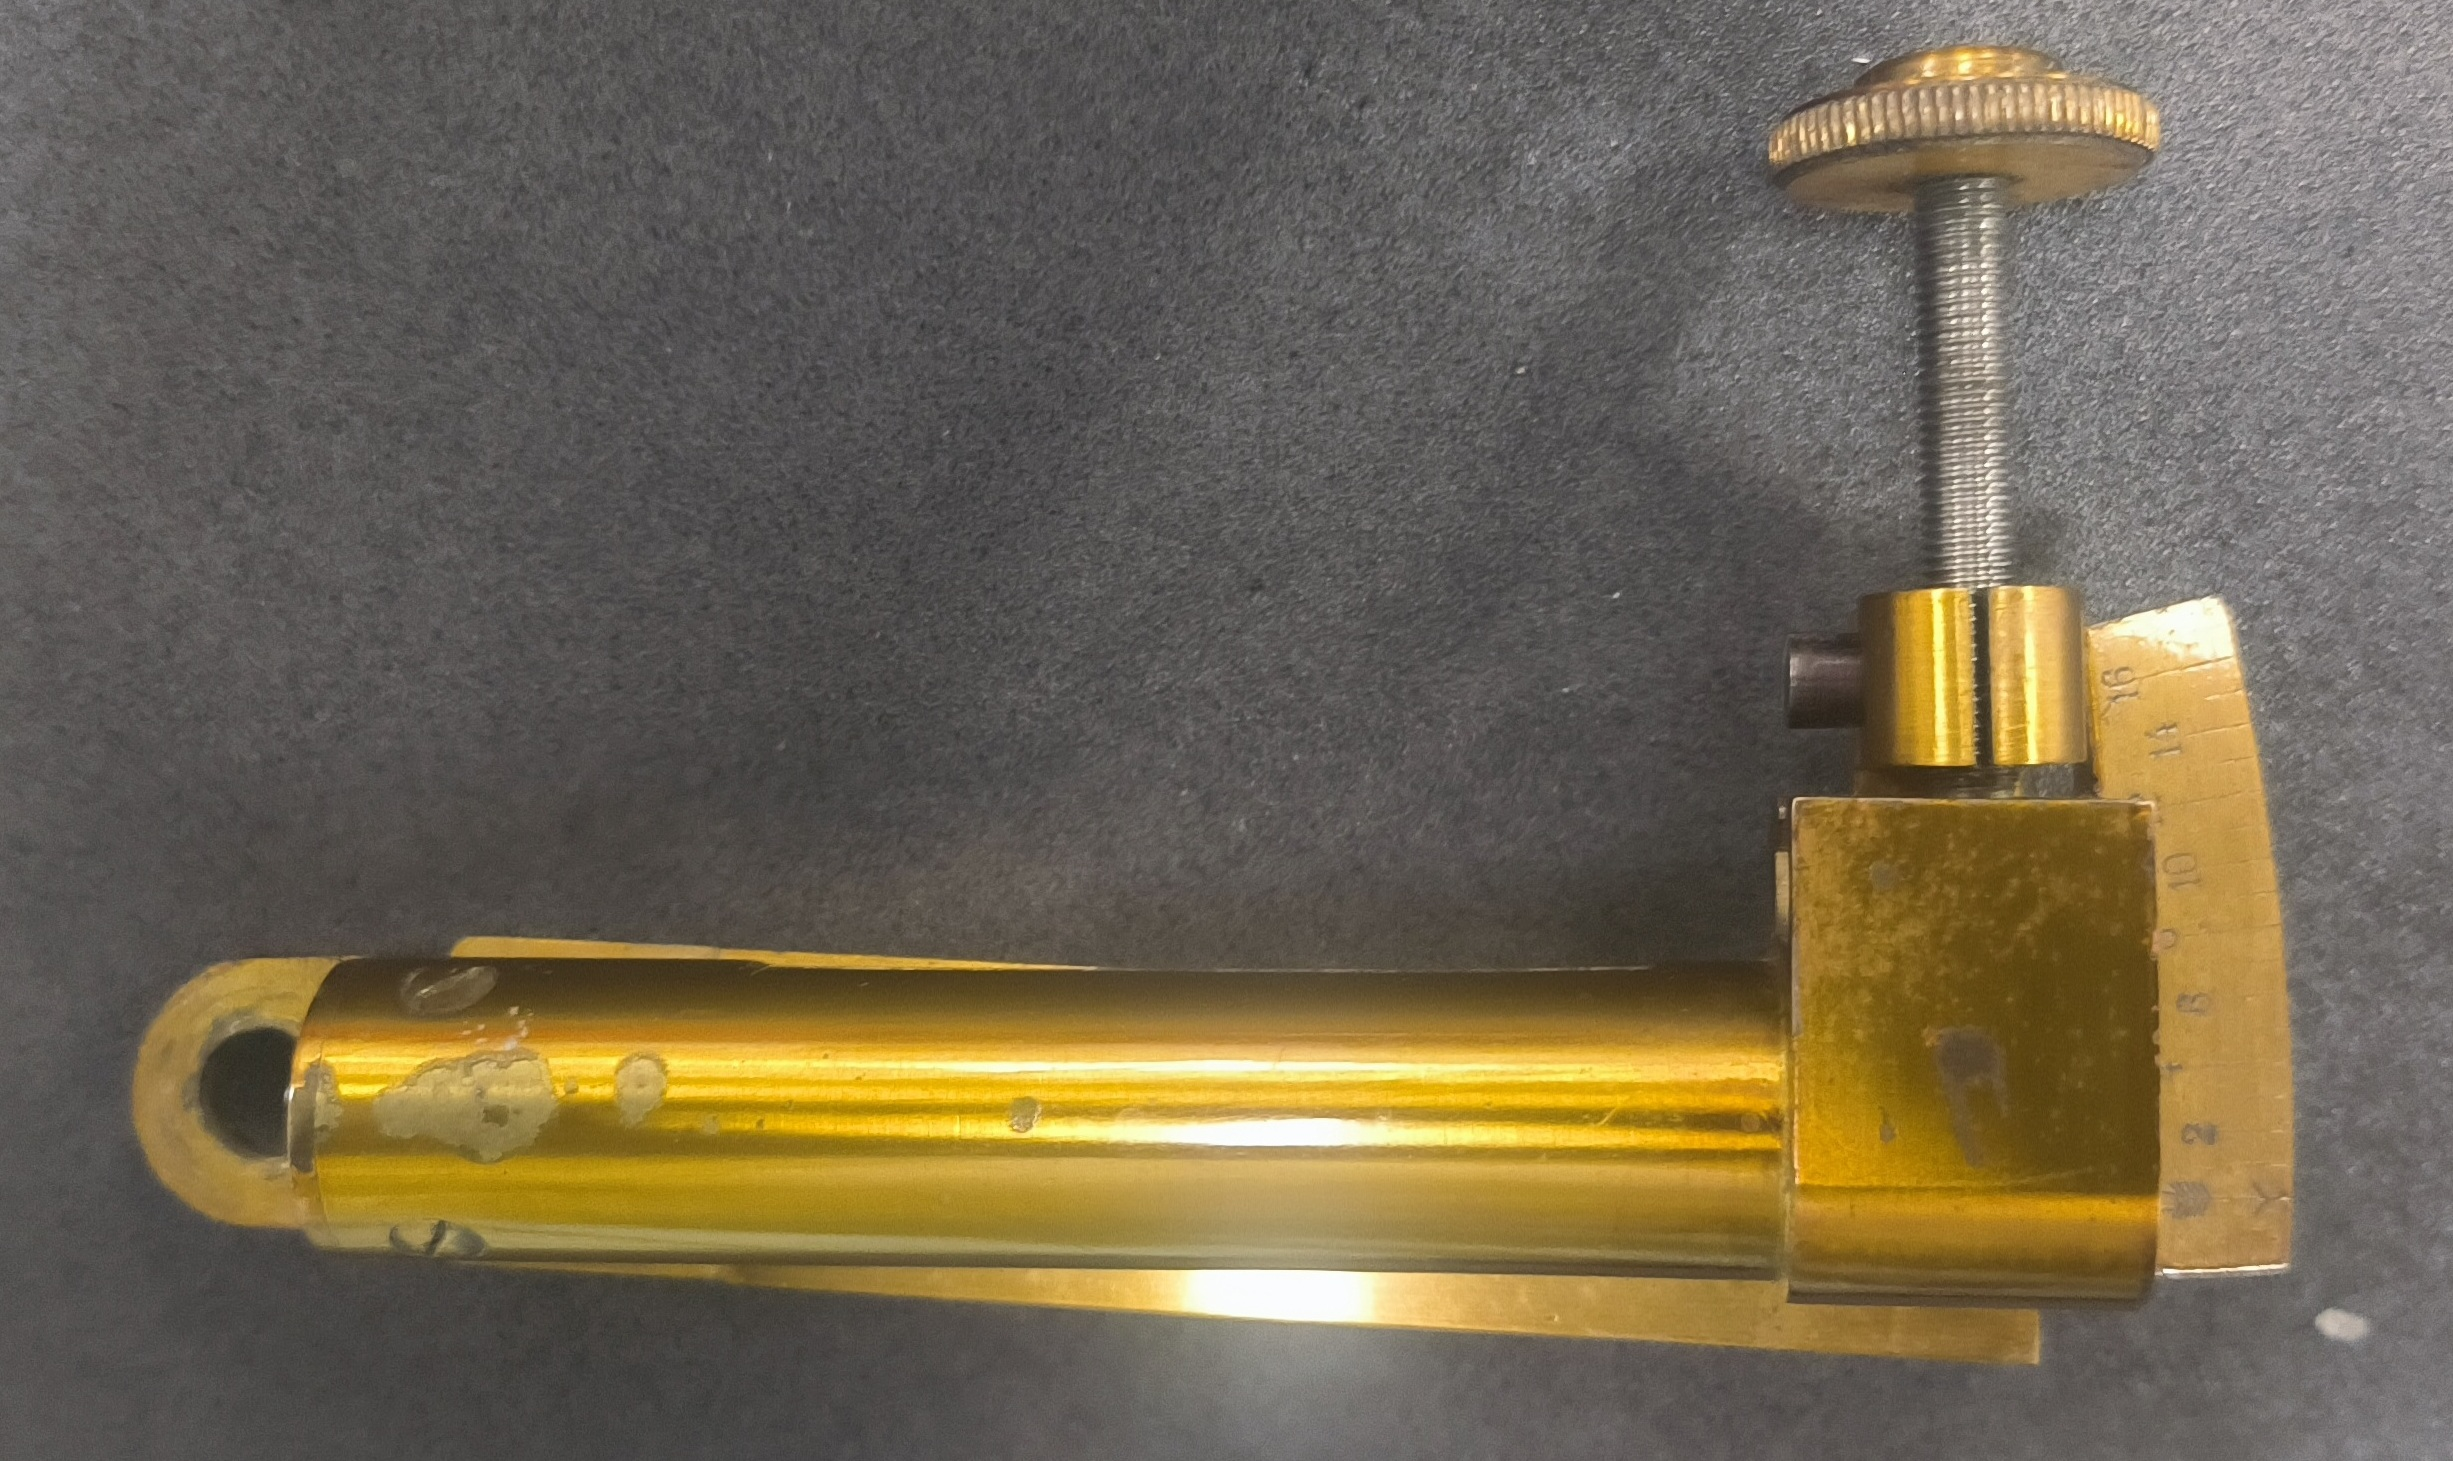
\includegraphics[width=0.9\textwidth]{img/vernier_structure_assembled.jpg}
        \caption{拼接后}
        \label{fig:vernier_structure_assembled}
    \end{minipage}
\end{figure}

游标底座贴合量盘的一面刻着“1113”,且包含一个螺丝,用于与位于量盘背部的活动的垫片及螺帽连接。游标底座上方有一个攻丝孔,内嵌螺丝,用于微调游标本体的角度。攻丝孔旁有一个小螺丝,可以用于调整攻丝孔的大小及松紧程度。

游标本体贴合游标底部的一面亦刻着“1113”。游标本体内嵌一个用于测量水平的玻璃管。经过测试可以分辨出1/16°的角度变化。

此外,也有部分测量的尺寸:背部的螺帽直径为 20.9mm,游标底座上方的螺丝顶部直径为 15.1mm,圆柱形玻璃管的之间为 12.5mm。

\section{仪器原理}

\subsection{游标读数}

该仪器在设计的时候利用了游标读数的原理,用于提高测量的精度,故通过解释游标卡尺的原理来介绍仪器的原理。游标卡尺是一种高精度测量工具,其读数原理基于游标尺与固定尺的刻度差。通常,游标尺的刻度会比固定尺的刻度稍小。以20个刻度的游标卡尺为例:固定尺的每个刻度为1毫米,而游标尺上20个刻度的总长度为19毫米,这样游标尺的每个刻度为0.95毫米。通过这种设计,可以实现精确的读数。

\begin{enumerate}
    \item \textbf{读取主尺读数}:找到游标零刻度对齐的主尺刻度。这是测量的基础值,称为主尺读数。
    \item \textbf{读取游标读数}:找到与固定尺上的刻度对齐的游标刻度。由于每个游标刻度为0.05毫米(1毫米 - 0.95毫米),对齐的游标刻度乘以0.05毫米即为游标读数。
    \item \textbf{计算总读数}:将主尺读数与游标读数相加,即得到最终的测量结果。
\end{enumerate}

如图\ref{fig:vernier_caliper},如果主尺读数为24毫米,而游标尺上第14个刻度对齐,则游标读数为14$\times$0.05毫米(假设每个游标刻度为0.05毫米),即0.70毫米。因此,总读数为24.70毫米。\cite{Vernier-scale}

\begin{figure}[h]
    \centering
    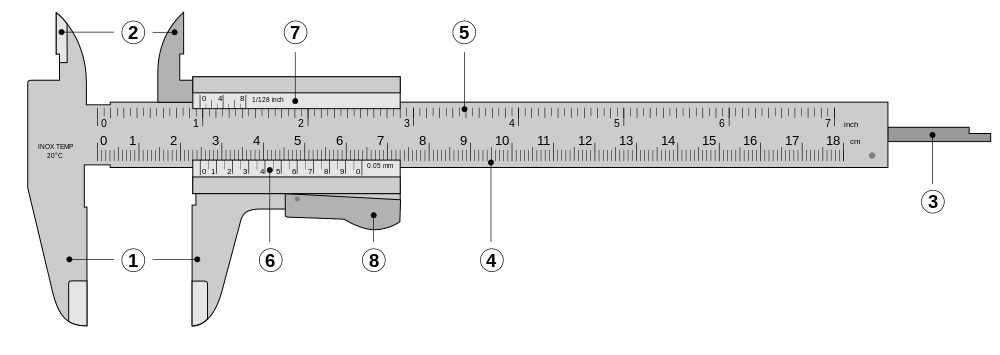
\includegraphics[width=0.8\textwidth]{img/vernier_caliper.png}
    \caption{游标卡尺示意图}
    \label{fig:vernier_caliper}
\end{figure}

\subsection{水平仪}

如图\ref{fig:bubble_level}当水平仪的底平面与水平位置有微小的差别时,也就是水平仪底平面两端有高低时,水准器内的气泡由于地心引力的作用总是往水准器的最高一侧移动,这就是水平仪的使用原理。 两端高低相差不多时,气泡移动也不多,两端高低相差较大时,气泡移动也较大,在水准器的刻度上就可读出两端高低的差值。\cite{bubble-level}

\begin{figure}[h]
    \centering
    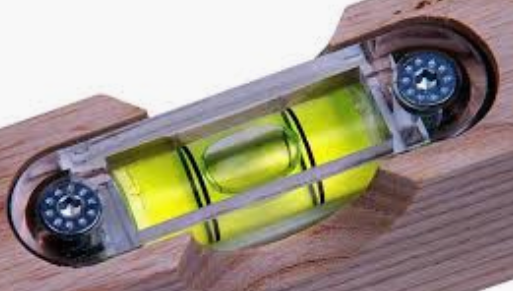
\includegraphics[width=0.5\textwidth]{img/bubble_level.png}
    \caption{水平仪示意图}
    \label{fig:bubble_level}
\end{figure}

\subsection{使用方法}

如图\ref{fig:clinometer_usage_adjust},在使用仪器时,需要将仪器竖立放置。首先粗调游标(按照绿色箭头所示。绕着左方螺丝旋转),使其游标与地面接近平行,再细调游标(旋转蓝色框内的旋钮),使得玻璃管内的液体泡位于中心(如图\ref{fig:clinometer_usage_judge}),此时游标与地面平行。最后按照游标卡尺的读数方式,读取游标尾部的刻度所对应的角度,即可得到测量结果。

\begin{figure}[h]
    \centering
    \begin{minipage}[t]{0.4\textwidth}
        \centering
        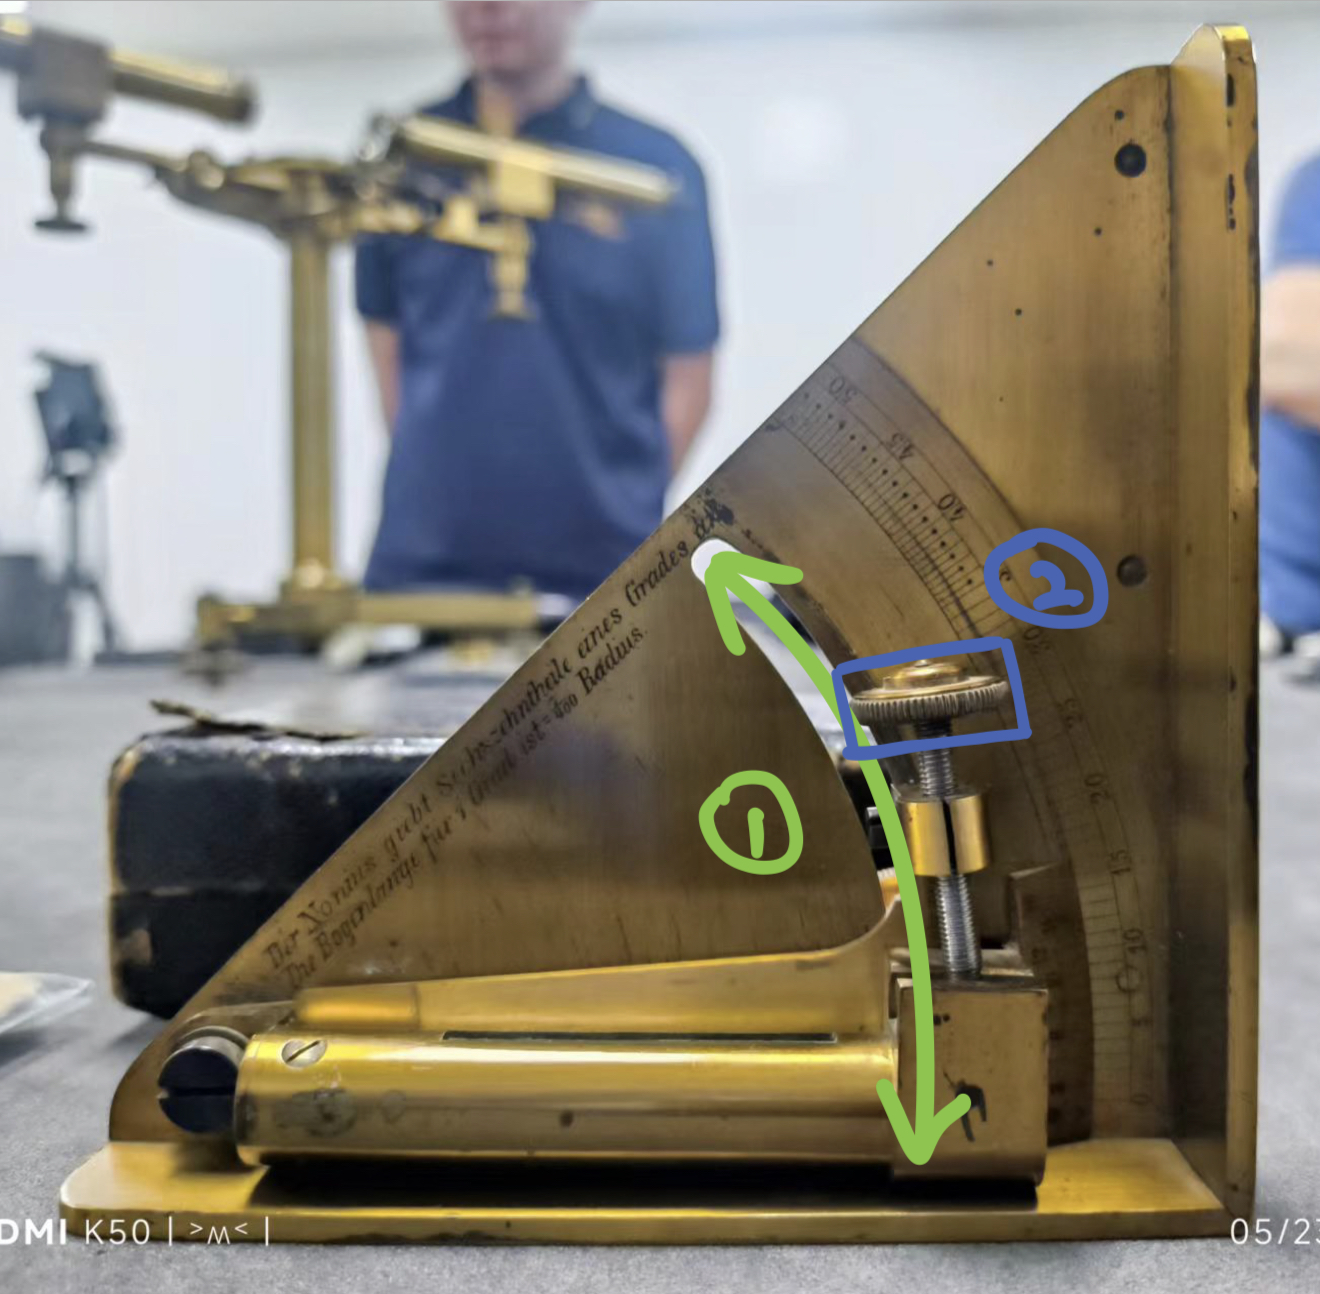
\includegraphics[width=0.8\textwidth]{img/clinometer_usage_adjust.jpg}
        \caption{测斜仪使用示意图}
        \label{fig:clinometer_usage_adjust}
    \end{minipage}
    \begin{minipage}[t]{0.5\textwidth}
        \centering
        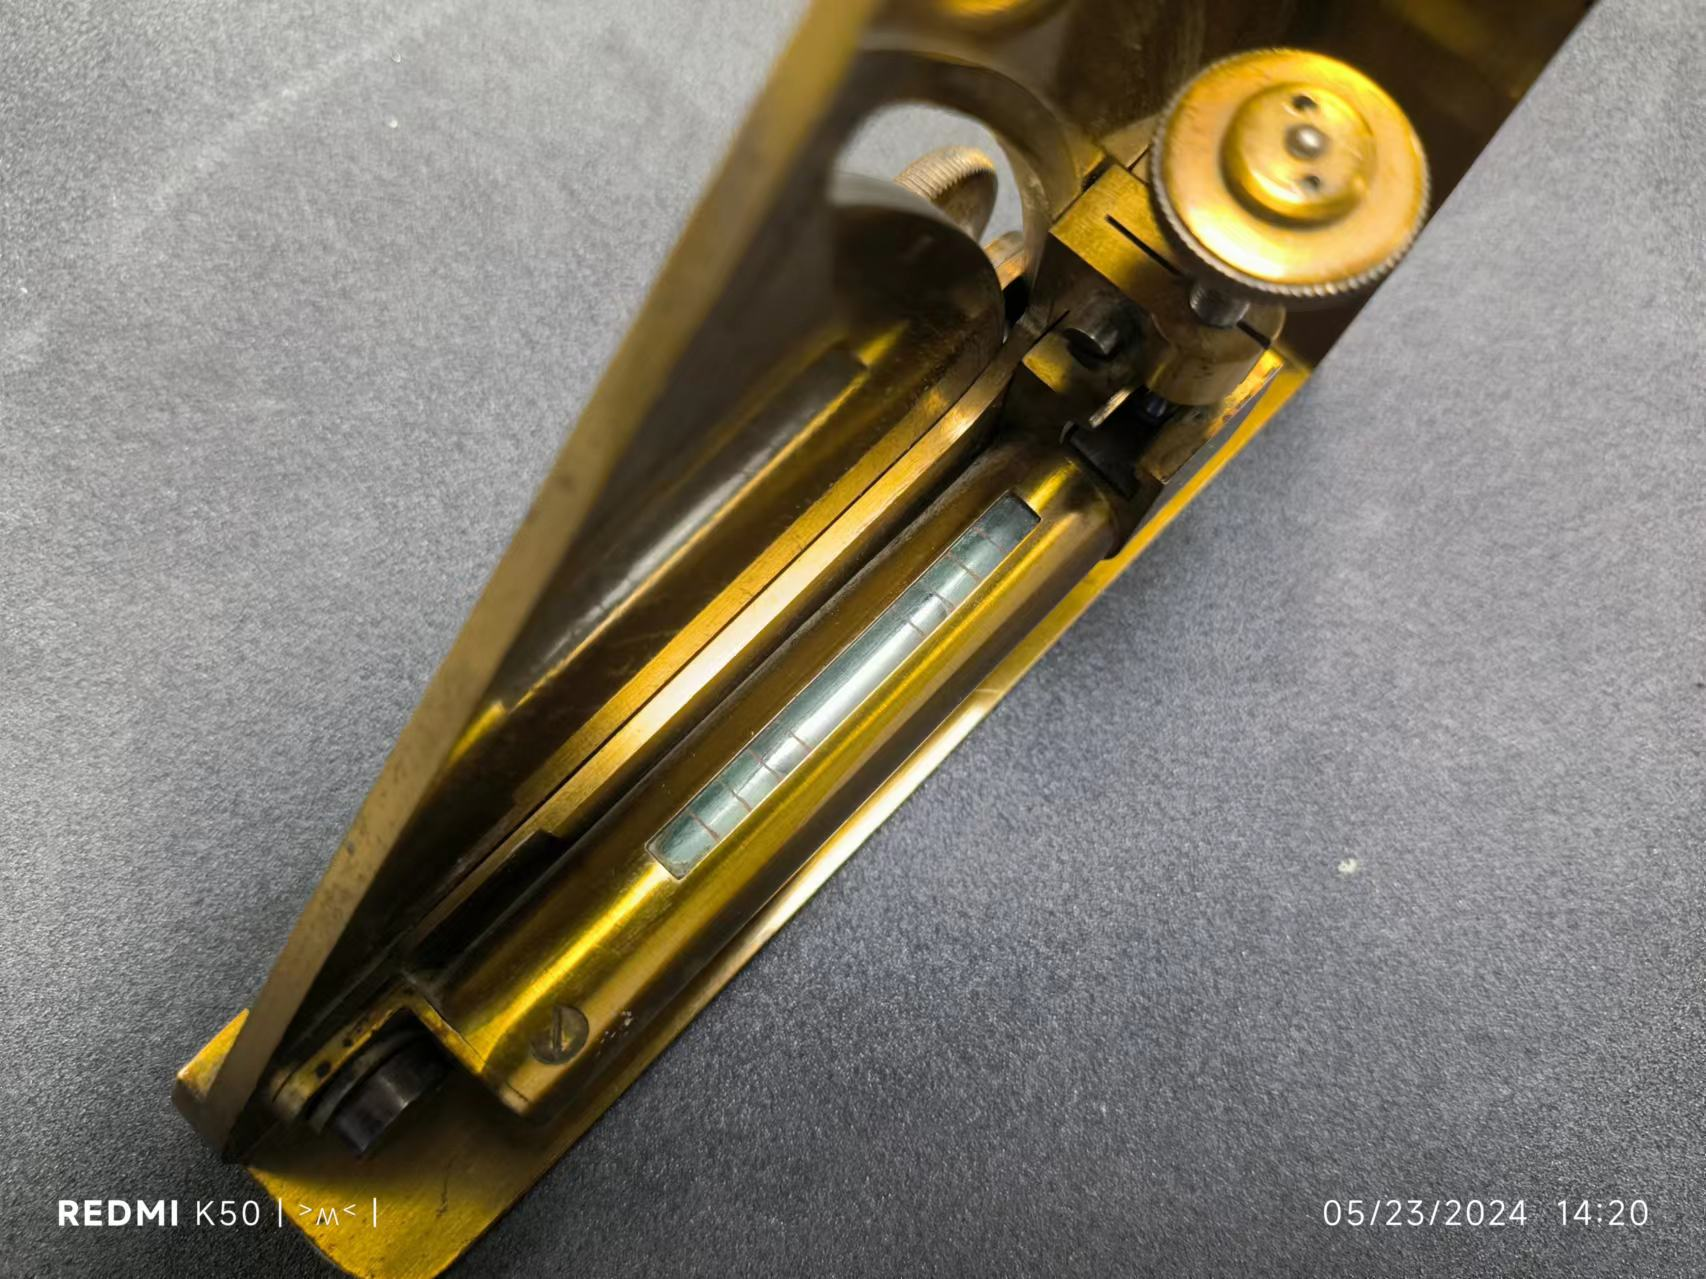
\includegraphics[width=0.84\textwidth]{img/clinometer_usage_judge.jpg}
        \caption{测斜仪水平判断}
        \label{fig:clinometer_usage_judge}
    \end{minipage}
\end{figure}

\section{相关资料}

\subsection{制作者与制作时间}

根据已有资料,W. Bandermann ,德国人,是一名数学仪器的制作者\cite{W-Bandermann},对火炮技术有突出贡献。根据对 W. Bandermann 和对测斜仪的记载,推测该仪器制作时间约为 1850-1900 年之间。

\subsection{仪器的来源与发展}

测斜仪的前身应该为炮手象限仪,这种仪器在 1537 年左右被 Nicolo Tartagli 设计,并发表在 \emph{Nova Scientia} 中\cite{doi:10.1080/00033799100200321}\cite{stanley1994quadrant}。

尼科洛-方塔纳-塔尔塔利亚(Niccolò Fontana Tartaglia,约 1499 - 1557 年 12 月 13 日)是意大利数学家、工程师和测量师,因其对数学和力学的贡献而闻名。塔尔塔利亚被认为是弹道学领域的先驱之一。他撰写了多篇关于射弹运动的论文,解决了与火炮和防御工事有关的实际问题。他的著作《新科学》(1537 年)为弹丸运动的科学研究奠定了基础。

如图\ref{fig:Nova_Scientia}所示,这种炮手象限仪使用重力作为测量的基准,通过测量铅锤与火炮的夹角来确定火炮的仰角。这种仪器的精度较低,但是在当时的技术水平下已经是一种很好的测量仪器。而图\ref{fig:gunner's_quadrant_front}与图\ref{fig:gunner's_quadrant_back}则是这一类仪器的图片。

\begin{figure}[h]
    \centering
    \begin{minipage}[t]{0.4\textwidth}
        \centering
        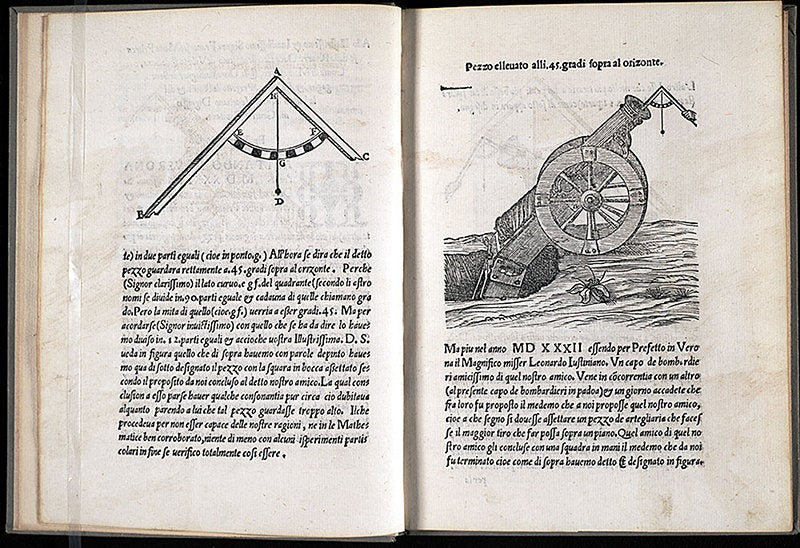
\includegraphics[width=1.0\textwidth]{img/Nova_Scientia.jpg}
        \caption{\emph{Nova Scientia}}
        \label{fig:Nova_Scientia}
    \end{minipage}
    \begin{minipage}[t]{0.28\textwidth}
        \centering
        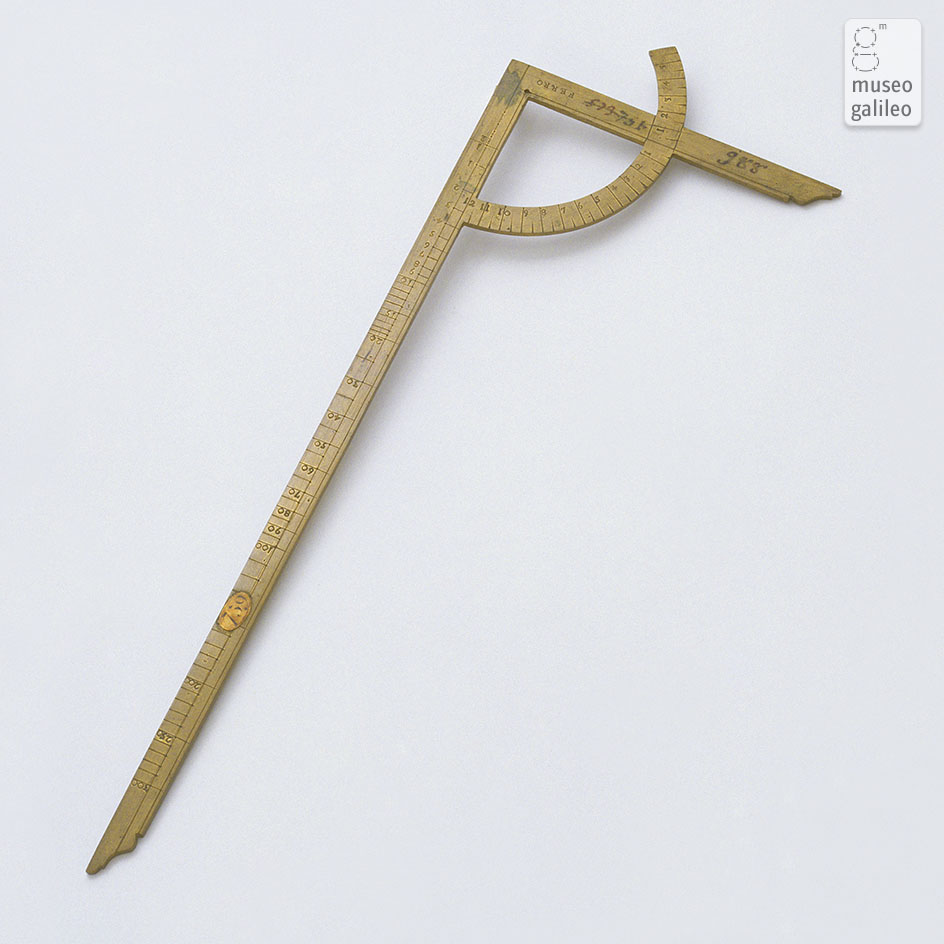
\includegraphics[width=1.0\textwidth]{img/gunners_quadrant_front.jpg}
        \caption{炮手象限仪正面}
        \label{fig:gunner's_quadrant_front}
    \end{minipage}
    \begin{minipage}[t]{0.28\textwidth}
        \centering
        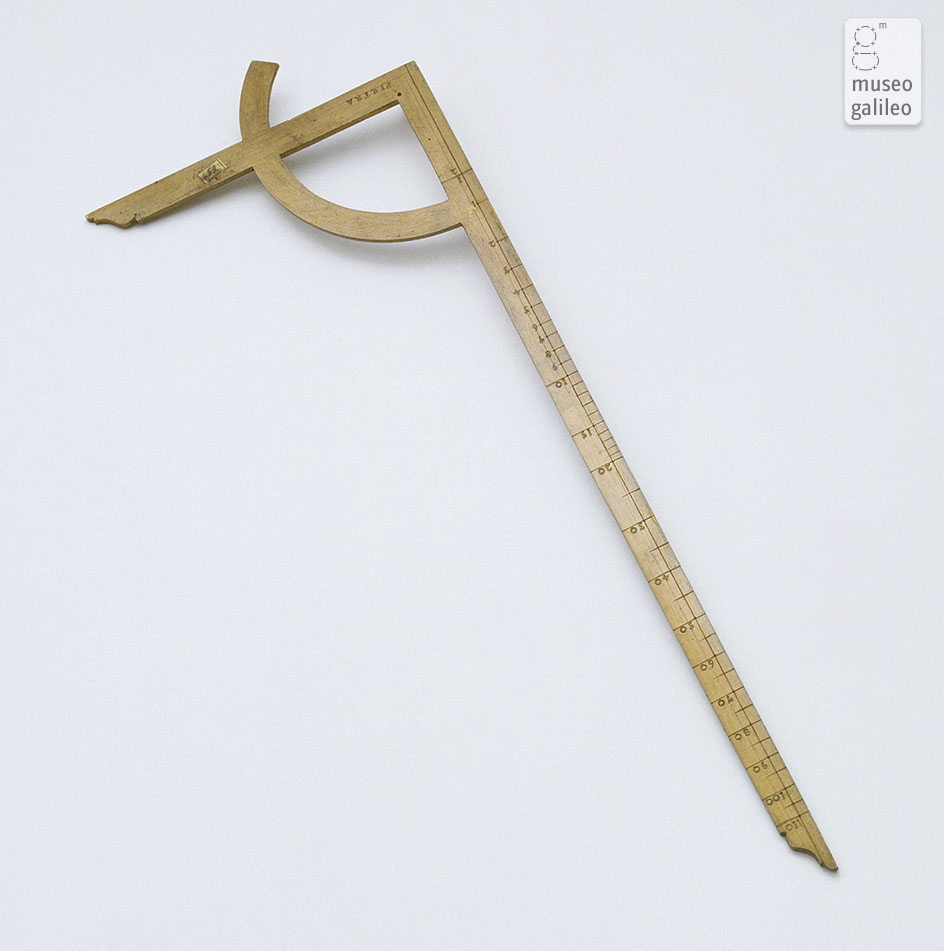
\includegraphics[width=1.0\textwidth]{img/gunners_quadrant_back.jpg}
        \caption{炮手象限仪背面}
        \label{fig:gunner's_quadrant_back}
    \end{minipage}
\end{figure}

在与 W. Bandermann 同一时期,出现了很多类似的测斜仪器,但是测量精度都不高,如图\ref{fig:John_Cail_clinometer}为John Cail制造的测斜仪\cite{Society1983}。但是,W. Bandermann 为测斜仪添加了游标,大幅度提高了测量的精度。这就是他的测斜仪的创新之处。

\begin{figure}[h]
    \centering
    \begin{minipage}[t]{0.4\textwidth}
        \centering
        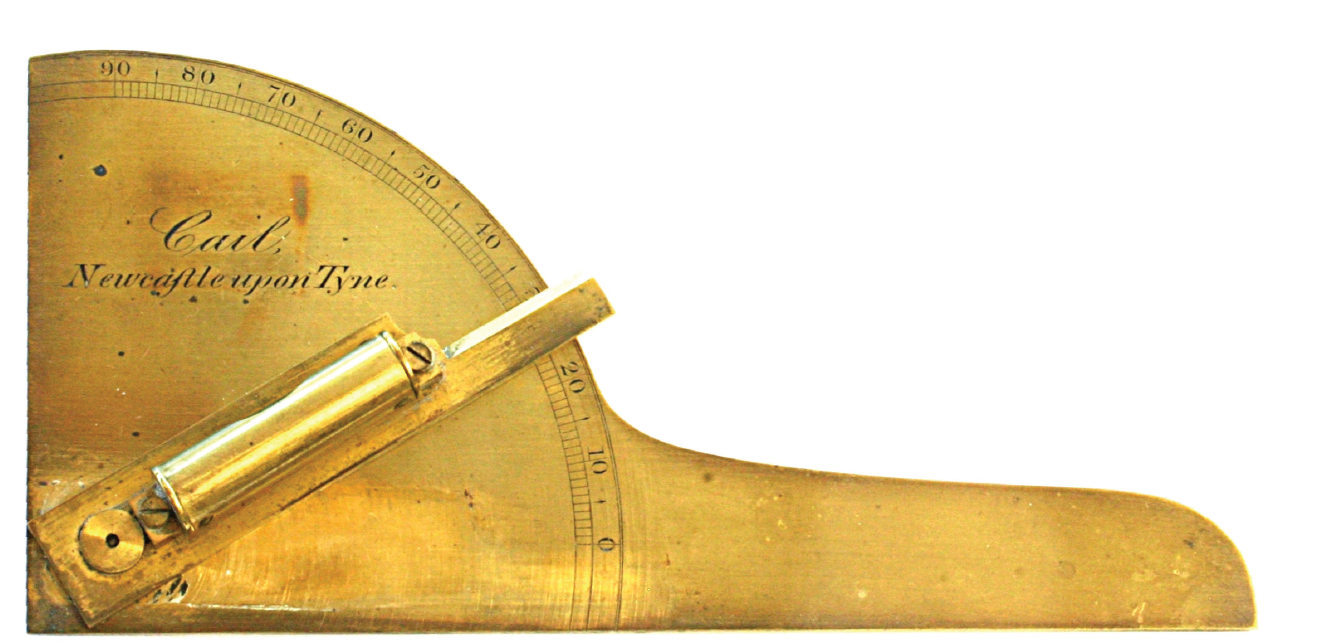
\includegraphics[width=1.0\textwidth]{img/John_Cail_clinometer.png}
        \caption{John Cail制造的测斜仪}
        \label{fig:John_Cail_clinometer}
    \end{minipage}
\end{figure}

除了文章中研究的仪器之外,W. Bandermann 也制造了几乎完全一致的测角度仪器,但是游标的分度为 1/4°,而非 1/16°\cite{Clinometer},如图\ref{fig:clinometer-1_4}。在之后的在第一次世界大战中,出现了由 Simson \& Co, Suhl 制作的改进版测量仪\cite{Artillery-clinometer},如图\ref{fig:Artillery-clinometer}。在第二次世界大战中,则出现了更加实用的的测斜仪,如M1炮手象限仪,如图\ref{fig:M1-clinometer}。

\begin{figure}[h]
    \centering
    \begin{minipage}[t]{0.3\textwidth}
        \centering
        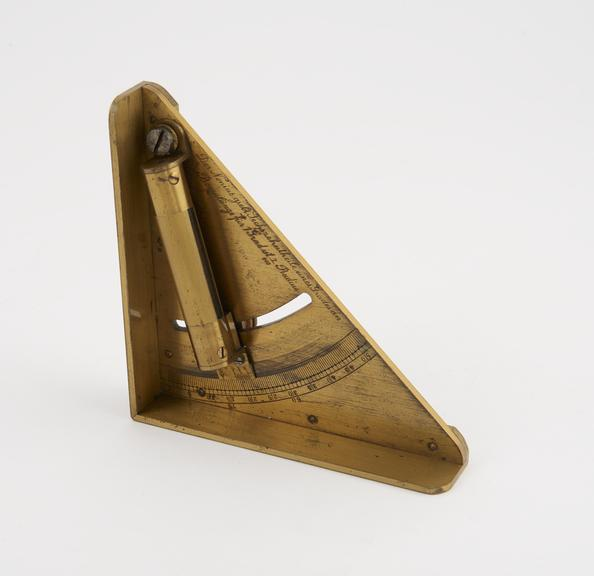
\includegraphics[width=0.93\textwidth]{img/clinometer-1_4.jpg}
        \caption{分度为1/4°测斜仪}
        \label{fig:clinometer-1_4}
    \end{minipage}
    \begin{minipage}[t]{0.3\textwidth}
        \centering
        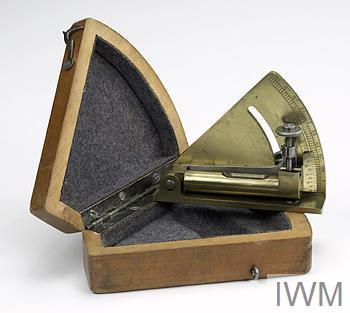
\includegraphics[width=1.0\textwidth]{img/Artillery-clinometer.png}
        \caption{改进后的测斜仪}
        \label{fig:Artillery-clinometer}
    \end{minipage}
    \begin{minipage}[t]{0.3\textwidth}
        \centering
        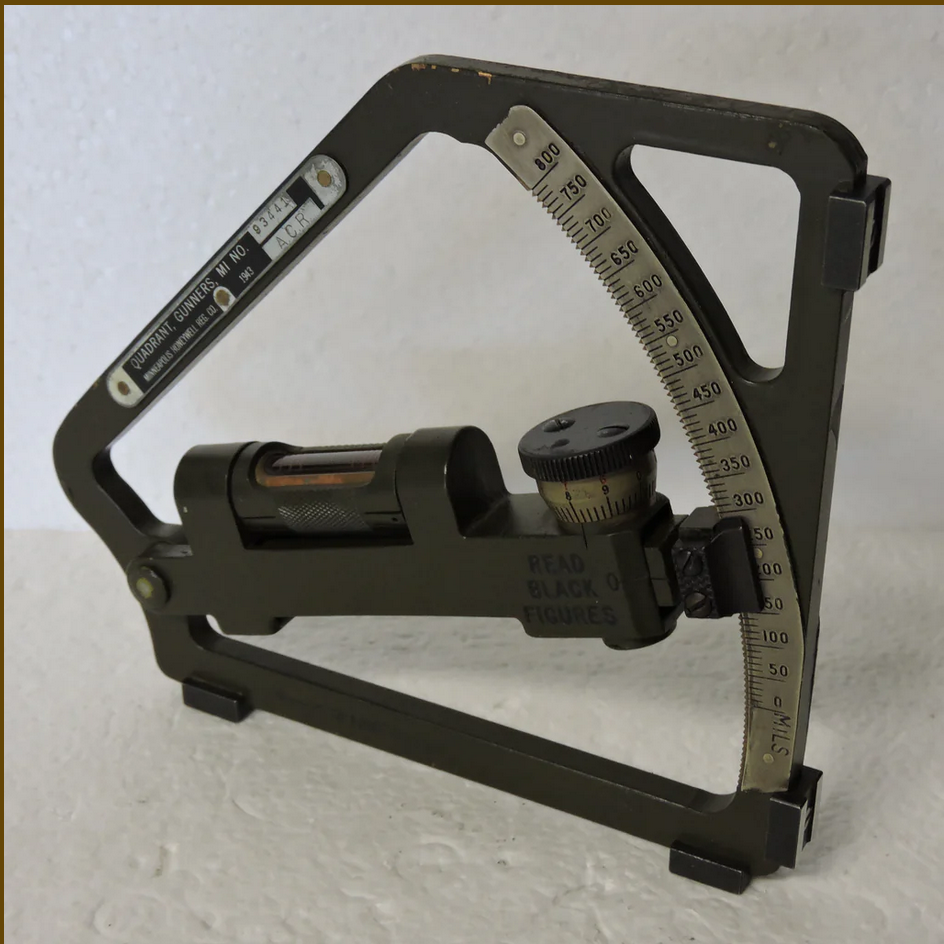
\includegraphics[width=0.9\textwidth]{img/M1-clinometer.png}
        \caption{M1测斜仪}
        \label{fig:M1-clinometer}
    \end{minipage}
\end{figure}

\subsection{仪器的意义与影响}

测斜仪在军事和工程领域具有重要意义。军事上,测斜仪大大提高了火炮的瞄准精度,充分发挥了火炮的射程和威力。历史上,没有测斜仪时,因为炮手无法准确瞄准目标,尽管火炮的射程可达10000码,海上交战的有效战斗距离约为1000码,火炮的射程优势难以利用。然而,有了测斜仪,炮手能够准确掌握敌人的位置,在更远的距离上击败敌人,从而提高了火炮的作战效果和射程。\cite{RangeFindersByGleaves1892}

此外,测斜仪对舰队作战战术也产生了深远影响。它使得远距离战斗成为可能,减少了船只冲撞和纠缠的近战场面,提高了战斗的精确性和致命性。这种战术变化使得舰队作战更注重火力和精确度,改变了海军战斗的传统方式。\cite{RangeFindersByGleaves1892}

在工程领域,测斜仪用于测量地面和建筑物的斜度,帮助工程师设计和建造稳定的结构。W. Bandermann制造的测斜仪以其高精度和便携性,广泛应用于多个领域,为工程测量提供了可靠的工具。

事实上,W. Bandermann的测斜仪不仅在当时发挥了重要作用,也为后来的测量仪器发展奠定了基础。它的设计和制造标准为后来的测斜仪提供了参考,为测量技术的发展做出了贡献。

\bibliographystyle{plain}
\bibliography{cite.bib}

\end{document}
